%! Author = Gianni
%! Date = 17/10/2023

% Preamble
\documentclass[a4paper,12pt]{report}

% Packages
\usepackage[italian]{babel}
\usepackage[left=3cm,right=3cm,top=2.3cm,bottom=3.5cm]{geometry}
\usepackage{listings, lstautogobble}
\usepackage{xcolor}
\usepackage{dirtree}
\usepackage{graphicx}
\usepackage{amsmath}
\usepackage{hyperref}
\usepackage[utf8]{inputenc}
\usepackage[T1]{fontenc}
\usepackage{ifthen}

\usepackage{breakurl}
\def\UrlBreaks{\do\/\do-}

%! Author = Gianni
%! Date = 12/12/2023

% Config package listings
\lstdefinelanguage{bash}{
    basicstyle=\small\ttfamily,
    numbers=left,
    numberstyle=\tiny,
    stepnumber=1,
    numbersep=8pt,
    showstringspaces=false,
    breaklines=true,
    frame=lines,
    backgroundcolor=\color{gray!10},
    tabsize=3,
    keywordstyle=\color{blue},
    morestring=[b],
    morecomment=[l]{//},
    morecomment=[s]{/*}{*/},
    autogobble=true
}
\lstdefinelanguage{python}{
    basicstyle=\small\ttfamily,
    numbers=left,
    numberstyle=\tiny,
    stepnumber=1,
    numbersep=8pt,
    showstringspaces=false,
    breaklines=true,
    frame=lines,
    backgroundcolor=\color{yellow!10},
    tabsize=3,
    keywordstyle=\color{blue},
    morestring=[b],
    morecomment=[l]{//},
    morecomment=[s]{/*}{*/},
    autogobble=true
}
\lstdefinelanguage{html}{
    basicstyle=\small\ttfamily,
    numbers=left,
    numberstyle=\tiny,
    stepnumber=1,
    numbersep=8pt,
    showstringspaces=false,
    breaklines=true,
    frame=lines,
    backgroundcolor=\color{green!10},
    tabsize=3,
    keywordstyle=\color{blue},
    morestring=[b],
    morecomment=[l]{//},
    morecomment=[s]{/*}{*/},
    autogobble=true
}
\lstdefinelanguage{text}{
    basicstyle=\small\ttfamily,
    numbers=left,
    numberstyle=\tiny,
    stepnumber=1,
    numbersep=8pt,
    showstringspaces=false,
    breaklines=true,
    frame=lines,
    backgroundcolor=\color{cyan!10},
    tabsize=3,
    keywordstyle=\color{blue},
    morestring=[b],
    morecomment=[l]{//},
    morecomment=[s]{/*}{*/},
    autogobble=true
}
\lstdefinelanguage{textnonum}{
    basicstyle=\small\ttfamily,
    showstringspaces=false,
    breaklines=true,
    frame=lines,
    backgroundcolor=\color{white},
    tabsize=3,
    keywordstyle=\color{blue},
    morestring=[b],
    morecomment=[l]{//},
    morecomment=[s]{/*}{*/},
    autogobble=true
}


\lstset{
    literate={{°}{\textdegree}1}
    }

\hypersetup{
    colorlinks=true,
    linkcolor=blue,
    citecolor=blue,
    filecolor=blue,
    urlcolor=blue
}

\newcommand{\reportitle}[1]{\renewcommand{\reportitle}{#1}}

\newcommand{\mytoc}{
    \tableofcontents
    \newpage
    \listoffigures
    \newpage
}

\newboolean{isThesis}
\setboolean{isThesis}{true}

%Document
\begin{document}

\reportitle{Sviluppo di un'architettura in cloud per la virtualizzazione di sensori e modelli di crescita in agricoltura}

%! Author = Gianni
%! Date = 12/12/2023

\begin{titlepage}

    \centering
    {\scshape\LARGE Università degli Studi di Verona \par}
    \vspace{1.5cm}
    \textsc{\Large Dipartimento di informatica}\\[0.5cm]
    \textsc{\large Laurea Triennale - Informatica}\\[0.5cm]
    \vspace{1.5cm}

    \rule{\linewidth}{0.35 mm} \\[0.4 cm]
    {\huge \bfseries \reportitle \par} \
    \rule{\linewidth}{0.35 mm} \\[1.5 cm]
    \vspace{1cm}

    \ifthenelse{\boolean{isThesis}}
    {
    \begin{minipage}{0.5\textwidth}
        \begin{flushleft}
            \large
            \textit{Autore:}\\
            Gianni \textsc{Donadon}\\
            \textit{Matricola:}\\
            VR437200
        \end{flushleft}
    \end{minipage}
    ~
    \begin{minipage}{0.4\textwidth}
        \begin{flushright}
            \large
            \textit{Relatore:}\\
            Davide \textsc{Quaglia}\\
            \textit{Co-Relatore:}\\
            Elia \textsc{Brentarolli}
        \end{flushright}
    \end{minipage}
    }{
    \begin{minipage}{1\textwidth}
        \begin{flushleft}
            \large
            \textit{Autore:}\\
            Gianni \textsc{Donadon}\\
            \textit{Matricola:}\\
            VR437200
        \end{flushleft}
    \end{minipage}
    }

    \vfill\vfill\vfill
    {\large Anno accademico 2022-2023 \par}

\end{titlepage}

\mytoc

%! Author = Bomber
%! Date = 13/12/2023

\chapter*{Introduzione}
\addcontentsline{toc}{chapter}{\protect\numberline{}Introduzione}


Lo scopo di questo documento è fornire una guida 
per creare un'architettura di sensori e modelli di crescita basata su MQTT.
Il capitolo~\ref{ch:mqtt} spiega brevemente il protocollo MQTT 
e l'architettura publisher/subscriber. 
Il capitolo~\ref{ch:broker-mqtt} è dedicato all'installazione 
e alla configurazione del Broker MQTT Mosquitto.
Nel capitolo~\ref{ch:client-mqtt} viene spiegato come usare una libreria 
per implementare i Client MQTT e viene indicato come eseguirli automaticamente.
Nel capitolo~\ref{ch:flask-web-server} si affronta la struttura e il funzionamento
del progetto Flask fino al deployment.
Infine nel capitolo~\ref{ch:homeassistant} si mostra come configurare
Home Assistant per la visualizzazione dei dati.
Alla fine del documento sono presenti varie appendici 
che riportano codici e script rilevanti.



%! Author = Gianni
%! Date = 11/12/2023

\chapter{Il protocollo MQTT}
\label{ch:mqtt}

\section{Definizione e caratteristiche principali}
\label{sec:mqtt-definizione}
Message Queuing Telemetry Transport, abbreviato con la sigla MQTT, è un protocollo di messaggistica usato su
architetture con pattern publisher/subscriber.
Si tratta di un protocollo open-source che funziona sullo stack TCP/IP, ma può essere implementato anche su altri
stack come quello Bluetooth.
È stato pensato per le comunicazioni in cui è necessario usare le risorse e la banda disponibili in modo efficiente
e con un basso impatto energetico.
Infatti questo protocollo è molto popolare in ambito IoT, Internet of Things, per la sua implementazione leggera e viene
impiegato in vari casi come:
\begin{itemize}
    \item Raccolta dati da sensori e pubblicazione in un server.
    \item Pubblicazione di dati mission-critical direttamente da un sensore al dispositivo dell'utente.
    \item Configurazione remota di dispositivi IoT.
    \item Invio di configurazione o aggiornamenti a tutti i dispositivi connessi.
\end{itemize}

\begin{figure}[htp]
    \centering
    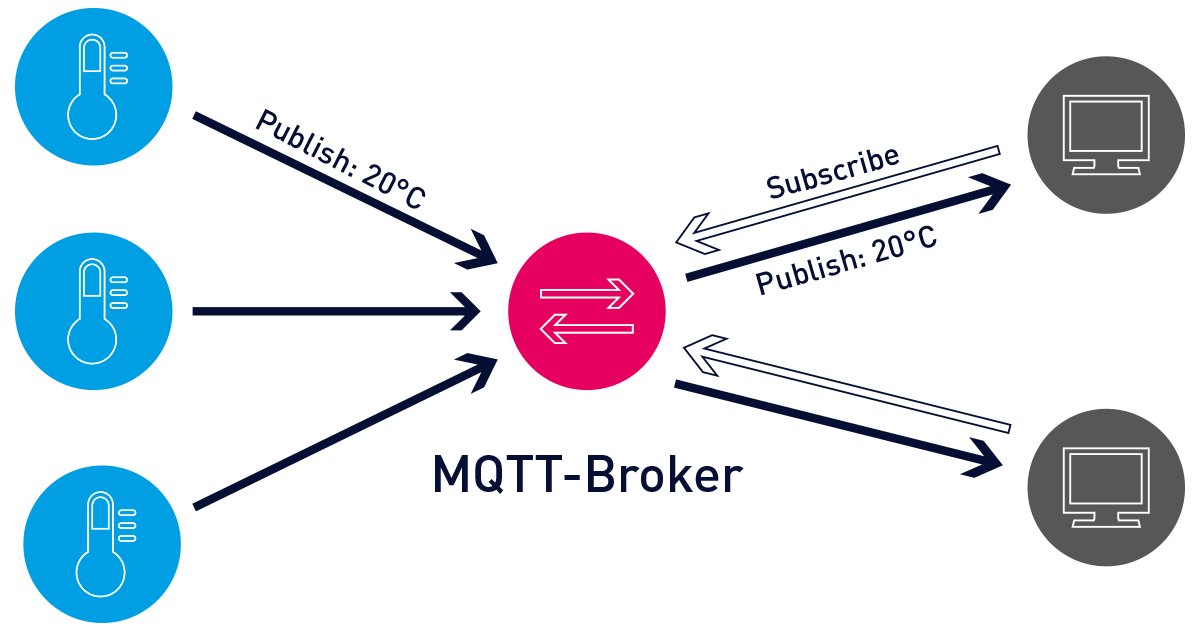
\includegraphics[width=0.7\linewidth]{images/chapter1-mqtt-architecture}
    \caption{Architettura Pub/Sub}
\end{figure}

%prima pagina
\section{L'architettura publisher/subscriber in MQTT}
\label{sec:mqtt-architettura}
Il modello architetturale publisher/subscriber si basa su tre componenti:
\begin{itemize}
    \item \textbf{Publisher}\newline
    Invia messaggi al broker.
    \item \textbf{Subscriber}\newline
    Richiede al broker di ricevere dei messaggi.
    \item \textbf{Broker}\newline
    Trasferisce i messaggi dai publisher ai subscriber.
\end{itemize}
I messaggi all'interno dell'architettura possono essere pubblicati in vari formati e possono essere filtrati in due modi:
in base al topic ("canale") oppure in base al contenuto.
Il filtro con topic prevede che i messaggi vengano categorizzati secondo dei canali.
Il publisher trasmette su un canale e il subscriber si deve iscrive a quel canale per ricevere solo quei messaggi.
Invece nel filtro con contenuto i messaggi non sono categorizzati.
I publisher inviano i messaggi e i subscriber definiscono un criterio con cui ricevere i messaggi. \newline
L'architettura permette il disaccoppiamento tra publisher e subscriber:
un publisher non conosce né gli altri publisher né i subscriber, e lo stesso vale per i subscriber.
Inoltre permette la comunicazione asincrona: il publisher non attende una risposta dopo l'invio.\newline
Nel caso specifico del protocollo MQTT, i messaggi sono organizzati secondo il filtro con topic
e vengono pubblicati in uno dei seguenti formati: JSON, XML, dati binari o testo.
I componenti assumono le seguenti denominazioni:
\begin{itemize}
    \item \textbf{Client publisher}\newline
    Pubblica sul broker messaggi su uno specifico topic.
    Questa operazione viene fatta da dispositivi come sensori.
    \item \textbf{Client subscriber}\newline
    Invia al broker la richiesta di iscrizione a uno o più topic.
    Questa operazione viene fatta da dispositivi che devono raccogliere o visualizzare i dati.
    \item \textbf{Broker MQTT}\newline
    È il sistema backend, chiamato impropriamente server, che coordina i diversi messaggi che arrivano dai client.
    Si può comparare a un ufficio postale che riceve i messaggi dai client "publisher" e li smista secondo un topic specifico.
    Successivamente li deve distribuire ai client "subscriber" iscritti a quel topic.
\end{itemize}
Un client in base alle funzioni che deve svolgere può essere publisher o subscriber oppure entrambi.




%! Author = Gianni
%! Date = 17/10/2023

\chapter{Broker MQTT Mosquitto}
\label{ch:broker-mqtt}

\section{Implementazione nel progetto}
\label{sec:broker-introduzione}
Alla base del progetto c'è il broker che permette la comunicazione tra le varie componenti.
Si è scelto di usare come broker Eclipse Mosquitto perché è open source e implementa il protocollo MQTT fino alla versione 5.0.
Di seguito viene spiegato come installare Mosquitto da terminale e come configurarlo per l'accesso locale e da remoto.
La guida è stata pensata per sistemi Linux.

\section{Installazione}
\label{sec:broker-installazione}

\subsection{Comandi per l'installazione}
L'installazione si può eseguire in più modi, come spiegato nel sito ufficiale \cite{mosquitto-install}:

\begin{itemize}
    \item \textbf{Metodo 1} - tramite la repository ufficiale (consigliato).\\
    In questo modo viene installata l'ultima versione disponibile delle release.
    \begin{lstlisting}[language=bash]
        sudo apt-add-repository ppa:mosquitto-dev/mosquitto-ppa
        sudo apt-get update
        sudo apt-get install mosquitto
    \end{lstlisting}
    \item \textbf{Metodo 2} - tramite la repository di linux.\\
    In questo modo viene installata l'ultima versione disponibile nel package manager.
    \begin{lstlisting}[language=bash]
        sudo apt-get install mosquitto
    \end{lstlisting}
\end{itemize}

\subsection{Come controllare l'esecuzione del servizio}
Il broker MQTT viene eseguito all'avvio della macchina tramite un servizio che viene aggiunto nell'installazione.
Il servizio si trova in:
\begin{lstlisting}[language=textnonum]
    /etc/systemd/system/mosquitto.service
\end{lstlisting}
È possibile controllare il broker con i consueti comandi per la gestione di un servizio elencati di seguito.
È necessario usare sudo, quindi si devono avere i diritti di root.
\begin{itemize}
    \item lo stato del servizio:
    \newline Solo questa opzione ha la possibilità di essere eseguita senza il comando sudo.
    \begin{lstlisting}[language=bash]
        sudo service mosquitto status
    \end{lstlisting}
    \item fermare il servizio:
    \begin{lstlisting}[language=bash]
        sudo service mosquitto stop
    \end{lstlisting}
    \item avviare il servizio:
    \begin{lstlisting}[language=bash]
        sudo service mosquitto start
    \end{lstlisting}
    \item riavviare il servizio:
    \begin{lstlisting}[language=bash]
        sudo service mosquitto restart
    \end{lstlisting}
\end{itemize}
Per vedere il log dettagliato di Mosquitto, si deve guardare nel file:
\begin{lstlisting}[language=textnonum]
    /var/log/mosquitto/mosquitto.log
\end{lstlisting}


\subsection{Problemi nell'installazione}
Si potrebbero presentare principalmente 2 tipi di problemi:
\begin{itemize}
    \item Mancata creazione della configurazione.\newline
    Vedere nella sezione~\ref{subsec:broker-esempi-configurazione} in cui si possono trovare esempi di configurazione.
    \item Nel caso di una precedente installazione:
    \begin{itemize}
        \item Si potrebbe avere un errore di database.\newline
        In questo caso si deve cancellare il database che si trova in:\\
        \textbf{var/lib/mosquitto/mosquitto.db} \newline
        Alla successiva esecuzione di Mosquitto questo database viene ricreato.
        \item Si potrebbero avere file di configurazione sbagliati o corrotti.\newline
        In questo caso si consiglia di creare un backup completo della cartella \textbf{/etc/mosquitto}.
        Eliminare tutti i file nella sotto cartella conf.d, rieseguire Mosquitto e vedere se funziona.
        Se il problema persiste eliminare anche il file con estensione .conf nella cartella mosquitto.
    \end{itemize}
\end{itemize}


\section{Configurazione}
\label{sub:broker-configurazione-del-broker}
Viene riportata la struttura della cartella contenente le configurazioni.
~\dirtree{%
    .1 /                (/etc/mosquitto/).
    .2 mosquitto.conf   (configurazione di default, da non modificare).
    .2 conf.d           (cartella per la configurazione .conf).
    .2 certs            (cartella per i certificati del server).
    .2 ca\_certificates  (cartella per i certificati della C.A.).
}

\subsection{Configurazione iniziale}
La configurazione del broker al momento dell'installazione è data dal file mosquitto.conf.
\newline
Se la cartella conf.d non contiene un file .conf viene caricata una configurazione di default
propria del broker. È impostata come segue:
\begin{lstlisting}[language=text]
listener 1883  #abilita il broker in ascolto alla porta 1883
allow_anonymous true #abilita l'accesso al broker a chiunque
\end{lstlisting}
Va sottolineato che con questa configurazione l'accesso al broker è abilitato a chiunque
e non ci sono restrizioni, perciò deve essere usato solo come ambiente di sviluppo.

\subsection{Configurazione parametri}
\label{subsec:broker-esempi-configurazione}
Può capitare che l'installazione non crei la struttura dei file e delle cartelle.
Si deve procedere a creare nella cartella \textbf{/etc/mosquitto} almeno il file
mosquitto.conf (si veda~\ref{sec:/mosquitto.conf}) e la cartella conf.d.\newline
Alcuni esempi di configurazione sono presenti in:
\begin{lstlisting}[language=textnonum]
    /usr/share/doc/mosquitto/examples
\end{lstlisting}
Per configurare il server in base alle proprie necessità, si deve creare un file con estensione .conf
all'interno della cartella conf.d. Questa sarà la configurazione che verrà caricata quando si eseguirà
il riavvio di Mosquitto.\newline
Di seguito vengono riportati alcuni parametri rilevanti che sono stati usati.
Si può fare riferimento alla documentazione ufficiale per la lista completa \cite{mosquitto-par-conf}.
\begin{itemize}
    \item \textbf{per\_listener\_settings [ true|false ]} :\label{table:broker-per-listener}\newline
    Abilita la gestione di autenticazione in modo differente per ogni listener.
    In questo modo si può avere, ad esempio, localhost senza password, mentre per l'accesso esterno serve
    l'autenticazione. Di default è False.
    \item \textbf{listener (port-number) [ip address/host name/unix socket path]} :\newline
    Dice a Mosquitto su quale porta mettersi in ascolto per le connessioni in entrata.
    Si deve specificare il numero della porta (le porte consigliate sono 1883 senza SSL e 8883 con SSL).
    Inoltre si deve associare il listener a un indirizzo ip o ad un host o ad un socket.
    Si possono definire più listener, uno per ogni porta, ed è possibile avere impostazioni diverse per ogni listener.
    Una volta definito un listener, le successive configurazioni sono associate a quel listener.
    \item \textbf{allow\_anonymous [ true|false ]} :\newline
    Determina se i client senza username sono abilitati alla connessione.
    Se è false si devono aggiungere configurazioni per il sistema di autenticazione.
    Viene associato ad un listener.
    Di default è False.
    \item \textbf{password\_file (file-path)} :\newline
    Imposta il percorso del password file.
    Il file contiene la coppia utente:password per ogni riga, con la password salvata come hash.
    È un primo metodo di autenticazione e si associa ad un listener.
    Per ulteriori dettagli si veda \ref{subsec:broker-password-file}.
    \item \textbf{certfile (file-path)} :\newline
    Imposta il percorso del certificato PEM del server.
    Viene usato insieme al parametro keyfile per abilitare la crittografia su TLS.
\end{itemize}
Nell'appendice~\ref{sec:/conf.d/localhost-tls.config} viene riporta la configurazione applicata al broker Mosquitto.
Sono presenti altri parametri che vengono spiegati successivamente.


\subsection{Metodi di autenticazione}
\label{sec:broker-autenticazione}
Come descritto nella guida ufficiale \cite{mosquitto-auth}, esistono 3 tipi di autenticazione:
\begin{itemize}
    \item unauthorized/anonymous access: nessun controllo.
    \item password files: gestione basilare.
    \item authentication plugins: controllo più avanzato.
\end{itemize}
Inoltre si possono avere differenti metodi di autenticazione per ogni listener, configurando più parametri listener,
\ref{table:broker-per-listener}.\newline
Nel progetto è stata usata l'autenticazione tramite \textit{password files} dato l'esiguo numero di account richiesti.


\subsubsection{Password file}
\label{subsec:broker-password-file}
Questo è un metodo semplice per gestire gli utenti in un singolo file,
tuttavia non è scalabile perché non permette la gestione puntuale di ogni client.
Inoltre richiede l'esecuzione di comandi dal terminale,
quindi è applicabile per casi non complessi come questo progetto.\newline
Questo metodo richiede le seguenti caratteristiche:
\begin{itemize}
    \item l'utente deve avere un nome univoco.
    \item la password deve essere immessa da terminale o in un file in chiaro.
    Una volta inserita viene salvato il suo hash.
    \item nel file di configurazione si devono applicare queste modifiche:
    \begin{itemize}
        \item \textbf{allow\_anonymous false} \newline
        Per disabilitare l'accesso anonimo e usare solo l'autenticazione utente e password.
        \item \textbf{password\_file /etc/mosquitto/nomefile} \newline
        Per dire al broker il percorso del file contente gli utenti e le password validi per quel listener.
    \end{itemize}
\end{itemize}
Per la creazione del file e degli utenti si possono eseguire i seguenti comandi:
\begin{itemize}
    \item \textbf{mosquitto\_passwd -c nomefile nomeutente} \newline
    Permette di creare nel percorso corrente un file con nome \textit{nomefile} e un utente con nome \textit{nomeutente}.
    Viene richiesto l'inserimento della relativa password. Questo metodo può essere usato per aggiungere un utente senza
    sovrascrivere il file se esiste già.
    \item \textbf{mosquitto\_passwd -b nomefile nomeutente password} \newline
    Permette l'aggiunta di un utente e della relativa password al file indicato.
    \item \textbf{mosquitto\_passwd -D nomefile nomeutente} \newline
    Permette l'eliminazione di un utente e della relativa password dal file indicato.
    \item \textbf{mosquitto\_passwd -U nomefile} \newline
    Dato un file in qualsiasi formato contenete utente e password in chiaro, uno per ogni riga,
    esegue l'hash delle password. È un metodo più veloce per aggiungere utenti.
\end{itemize}
Terminate le modifiche si deve ricaricare la configurazione del broker.
Per ricaricare la configurazione senza riavviare il servizio, si devono avere i diritti root:
\begin{lstlisting}[language=bash]
sudo pkill -HUP -x mosquitto
\end{lstlisting}
Per l'elenco completo dei comandi si guardi la documentazione di Mosquitto \cite{mosquitto-password}.
La guida che spiega come implementare la connessione al broker da parte di un client con autenticazione
è riportata nella sitografia finale \cite{mosquitto-password-1}.


\subsection{Certificati SSL/TLS}
\label{sec:broker-ssl-tls}
Il broker Mosquitto supporta l'autenticazione e la connessione criptata tramite SSL.\newline
È possibile generare dei certificati self signed, come spiegato nella documentazione \cite{mosquitto-ssl}.
Tuttavia si possono incontrare programmi o script che non gradiscono questo tipo di certificati, quindi
si deve optare per dei certificati di una vera CA, Certificate Authority.\newline
Si è optato per la configurazione dei certificati tramite la CA LetsEncrypt. Di seguito vengono spiegati
i vari passaggi di configurazione di \textit{certbot} per LetsEncrypt, per poi soffermarsi sul funzionamento
con il broker e i relativi problemi.\newline
Vengono riportate man mano varie fonti, dato che non è stato possibile trovare un'unica documentazione per risolvere
i problemi \cite{mosquitto-ssl-1} \cite{mosquitto-ssl-2} \cite{mosquitto-ssl-3}.

\subsubsection{Certbot}
Certbot è un tool che permette di gestire i certificati, le richieste e i rinnovi.
Per la creazione del certificato si deve avere l'accesso root alla macchina.
Inoltre, è necessario avere l'accesso alle impostazioni DNS del dominio associato alla macchina,
oppure, in alternativa, un web server sulla macchina in cui si installa Mosquitto.\newline
Si consiglia di seguire la documentazione per la corretta configurazione ad ogni passaggio \cite{mosquitto-ssl-1}.\newline
La procedura prevede:
\begin{enumerate}
    \item \textbf{Installazione Certbot}\newline
    Si esegue il comando:
    \begin{lstlisting}[language=bash]
    sudo apt-get -y install certbot
    \end{lstlisting}
    \item \textbf{Creazione di un certificato tramite DNS}\newline
    Il certificato che si crea è di tipo wildcard, quindi se il dominio è mydomain.it è valido anche per i sottodomini,
    così da poterlo usare per altri servizi.
    Il dominio DNS deve essere già associato alla macchina.
    Si esegue il comando:
    \begin{lstlisting}[language=bash]
    certbot certonly --manual --preferred-challenge dns -d *.mydomain.it
    \end{lstlisting}
    Si seguono le istruzioni a schermo, che prevedono l'aggiunta di un record DNS al dominio per validarlo.
    Al termine si ha generato dei certificati validi.
    \item \textbf{Rinnovo dei certificati}\newline
    Il rinnovo si può eseguire:
    \begin{itemize}
        \item \textbf{Manualmente}\newline
        Si esegue il comando:
        \begin{lstlisting}[language=bash]
            sudo certbot renew
        \end{lstlisting}
        \item \textbf{Automaticamente}\newline
        Si deve modificare il crontab per eseguire il comando di auto rinnovo periodicamente \cite{mosquitto-ssl-4}.
        Si esegue:
        \begin{lstlisting}[language=bash]
            sudo crontab-e
        \end{lstlisting}
        Poi si aggiungono alla fine del file le seguenti righe:
        \begin{lstlisting}[language=text]
            # Auto-renew let's encrypt SSL certificates
            0     *     *     *     *      sudo certbot renew
        \end{lstlisting}
    \end{itemize}
    \item \textbf{Accesso ai certificati}\newline
    Per accedere ai certificati si usano i symbolic link presenti nella cartella:
    \begin{lstlisting}[language=textnonum]
    /etc/letsencrypt/live/mydomain.it/
    \end{lstlisting}
    Non si accede direttamente ai certificati perché questi hanno una scadenza, di solito di alcuni mesi.
    Questi link sono mantenuti da Certbot e puntano all'ultima versione dei certificati.
\end{enumerate}

\subsubsection{Funzionamento con Mosquitto}
Mosquitto funziona sulla macchina con un utente che non ha i diritti root,
quindi non ha accesso alle cartelle dei certificati.
Tuttavia, seguendo le indicazioni fornite su Github dalla stessa Eclipse Mosquitto,
si riesce a copiare i certificati permettendo l'accesso a Mosquitto \cite{mosquitto-ssl-2}.
La procedura prevede:
\begin{enumerate}
    \item \textbf{Copia automatica dei certificati}\newline
    Lo script presente nell'appendice~\ref{sec:script-rinnovo-certificati} permette la copia e il cambio proprietario
    ad ogni rinnovo dei certificati.
    Lo script deve essere modificato nella riga 16, per specificare il dominio dei certificati interessati,
    e nella riga 18, per specificare la cartella di Mosquitto in cui si copieranno i certificati.
    Successivamente si copia lo script nella cartella (servono i diritti root):
    \begin{lstlisting}[language=textnonum]
    /etc/letsencrypt/renewal-hooks/deploy/
    \end{lstlisting}
    Si rende eseguibile lo script:
    \begin{lstlisting}[language=bash]
        sudo chmod +x /etc/letsencrypt/renewal-hooks/deploy/mosquitto-copy.sh
    \end{lstlisting}
    Con questa procedura Mosquitto ha ad ogni rinnovo dei certificati l'ultima versione.
    \item \textbf{Copia manuale dei certificati}\newline
    Probabilmente la prima volta si devono copiare manualmente i certificati.
    Si devono eseguire i seguenti comandi che fanno gli stessi passaggi dello script:
    \begin{lstlisting}[language=bash]
        # copia dei file
        sudo cp  /etc/letsencrypt/live/mydomain.it/fullchain.pem /etc/mosquitto/certs/fullchain.pem
        sudo cp  /etc/letsencrypt/live/mydomain.it/privkey.pem /etc/mosquitto/certs/privkey.pem
        # imposta l'owner a Mosquitto
        sudo chown mosquitto: /etc/mosquitto/certs/fullchain.pem /etc/mosquitto/certs/privkey.pem
        # imposta i diritti solo per Mosquitto
        sudo chmod 0600 /etc/mosquitto/certs/fullchain.pem /etc/mosquitto/certs/privkey.pem
        # dice a Mosquitto di ricaricare certificati e configurazione
        sudo pkill -HUP -x mosquitto
    \end{lstlisting}
    \item \textbf{Modifica configurazione Mosquitto}\newline
    Nella configurazione .conf di mosquitto si devono modificare 2 parametri impostando il path dei certificati:
    \begin{lstlisting}[language=bash]
        certfile /etc/mosquitto/certs/fullchain.pem
        keyfile /etc/mosquitto/certs/privkey.pem
    \end{lstlisting}
\end{enumerate}
Terminate queste modifiche Mosquitto può ricevere connessioni con TSL sul listener configurato.
I client che si connettono devono abilitare la connessione con TSL e opzionalmente la validazione del certificato.

\section{Disinstallazione}
\label{sub:broker-disinstallazione-del-broker}

\subsection{Eliminazione della configurazione}
\label{subsec:broker-eliminazione-configurazione}
Prima di procedere con la disinstallazione si consiglia di fare il backup delle configurazioni
e dei certificati presenti nelle rispettive cartelle.
Successivamente si consiglia di eliminare la cartella \textbf{/etc/mosquitto} per evitare futuri problemi.
Nel caso in cui siano stati configurati listener con TLS,
si deve eliminare lo script di copia automatica dei certificati.

\subsection{Rimozione del broker}
\label{subsec:broker-disinstallazione}
Per rimuovere la repository e l'installazione di Mosquitto si eseguono i seguenti comandi:
\begin{lstlisting}[language=bash]
sudo apt-add-repository --remove ppa:mosquitto-dev/mosquitto-ppa
sudo apt-get update
sudo apt-get remove mosquitto
sudo apt-get autoremove
\end{lstlisting}


%! Author = Gianni
%! Date = 08/02/2024

\chapter{Client MQTT}
\label{ch:client-mqtt}

\section{Implementazione nel progetto}
\label{sec:client-introduzione}
Ogni componente deve avere un client per comunicare tramite il broker.
Nel progetto è stata scelta come client la libreria python "paho-mqtt", in quanto viene sviluppata
dalla fondazione Eclipse, la stessa del broker Mosquitto.
Inoltre si è deciso di sviluppare i client con il linguaggio di programmazione Python,
perché è un linguaggio interpretato spesso usato per l'analisi di dati
e permette di eseguire il debug in modo semplice.
La seguente guida è stata pensata per sistemi Linux Ubuntu.

\section{Installazione}
\label{sec:client-installazione}

\subsection{Python}
\label{subsec:client-installazione-python}
Per poter procedere è necessario installare Python nel proprio sistema operativo.
Si consiglia di installare l'ultima versione di Python 3 supportata dal proprio sistema (si veda il sito ufficiale \cite{client-python}).
L'esecuzione di Python avviene dal terminale dei comandi o tramite script.
Si noti che, in base a come sono impostate le variabili di ambiente, 
python può essere eseguito con il nome "python" o "python3".
In base al sistema operativo in uso è possibile che Python sia già installato.
Per verificare la versione installata si procede con il seguente comando:
\begin{lstlisting}[language=bash]
	python3 -V
	# oppure
	# python -V
\end{lstlisting}
Se non risulta installato, nei sistemi Ubuntu si procede all'installazione con:
\begin{lstlisting}[language=bash]
	sudo apt install python3-pip
\end{lstlisting}
Successivamente si consiglia di chiudere e riaprire il terminale per usare le variabili di ambiente aggiornate.


\subsection{L'ambiente virtuale}
\label{subsec:client-installazione-ambiente-virtuale}
L'uso di un ambiente virtuale (virtual environment) è un aspetto spesso sottovalutato quando si programma in Python.
Un ambiente virtuale è isolato dall'installazione base di Python 
e ha una cartella propria in cui si trovano le dipendenze e le configurazioni per l'esecuzione del proprio codice.
In questo modo si possono avere diverse versioni di una libreria su diversi ambienti che sfruttano la stessa installazione Python.
Molto spesso la funzionalità dell'ambiente virtuale viene installata insieme a Python,
dato che dalla versione 3.3 di Python è stata introdotta nel modulo "venv" una versione basilare della libreria "virtualenv".
Per sfruttare a pieno le funzionalità della virtualizzazione si può installare la libreria "virtualenv" \cite{client-virtualenv},
ma per questo progetto è più che sufficiente quella integrata in Python.
Per verificare se la libreria è installata si procede con:
\begin{lstlisting}[language=bash]
	python3 -m venv
\end{lstlisting}
Se la libreria è già installata viene notificato un errore di mancanza di argomenti; in caso contrario si deve installare con:
\begin{lstlisting}[language=bash]
	sudo apt install python3-venv
\end{lstlisting}
Una volta terminata l'installazione si può procedere alla creazione di un ambiente, 
posizionandosi nella cartella in cui lo si vuole generare ed eseguendo: 
\begin{lstlisting}[language=bash]
	python3 -m venv venv
\end{lstlisting}
L'ultimo parametro è quello che specifica il path in cui verrà creato l'ambiente.
In questo caso si crea nella cartella corrente un ambiente chiamato "venv".
Una volta creato, si deve dire a Python di cambiare l'ambiente che sta usando.
Si procede con l'attivazione:
\begin{lstlisting}[language=bash]
	source venv/bin/activate
\end{lstlisting}
Questo comando richiama uno script all'interno dell'ambiente e attiva l'ambiente solo nel terminale corrente.
Da questo punto in poi tutto quello che si esegue modifica solo questo ambiente virtuale.
Si può procedere con l'installazione delle varie librerie e pacchetti.\newline
Per disattivare un ambiente e ritornare all'ambiente base di Python si esegue:
\begin{lstlisting}[language=bash]
	deactivate
\end{lstlisting}
Per eliminare un ambiente è sufficiente eliminare la cartella dell'ambiente virtuale.

\subsection{I requisiti}
\label{subsec:client-installazione-requisiti}
Spesso nei progetti Python si ha a disposizione un file denominato "requirements" (requisiti), 
in cui è presente la lista delle librerie e la versione usata dal progetto.
Per l'installazione dei requisiti si esegue:
\begin{lstlisting}[language=bash]
	python3 -m pip install -r requirements.txt
\end{lstlisting}
In questo modo nell'ambiente virtuale sono installati tutti i componenti 
che il progetto richiedeva quando è stato sviluppato.
Da questo punto in poi si è pronti a eseguire il progetto.\newline
Per salvare la lista delle dipendenze del corrente ambiente si usa il comando:
\begin{lstlisting}[language=bash]
	python3 -m pip freeze > requirements.txt
\end{lstlisting}

\subsection{La libreria paho-mqtt}
\label{subsec:client-installazione-libreria}
Si procede a installare la libreria come descritto nella documentazione ufficiale \cite{client-paho-doc-main},
nell'ambiente in cui si vuole eseguire il codice, con il seguente comando:
\begin{lstlisting}[language=bash]
	python3 -m pip install paho-mqtt
\end{lstlisting}
Viene installata la libreria nell'ultima versione compatibile con le varie dipendenze.
Ora è possibile creare dei client per interagire con il broker.\newline
Per rimuovere la libreria è sufficiente eseguire la disinstallazione: \label{python-rimuovere-libreria}
\begin{lstlisting}[language=bash]
	python3 -m pip uninstall paho-mqtt
\end{lstlisting}


\section{Le componenti del client}
\label{sec:client-creazione}
La libreria è formata principalmente da 3 moduli: client, publish e subscribe.
Il modulo "client" è quello completo che contiene tutto, dalla connessione alla pubblicazione e l'iscrizione.
I moduli "publish" e "subscribe" invece sono una versione semplificata della pubblicazione e dell'iscrizione,
quindi non ci sono tutte le funzionalità per gestire la connessione.\newline
Per il progetto è stato usato il modulo "client" per la creazione degli skeleton dei client
così da non avere limitazioni per futuri sviluppi.
Ci si è basati sulla documentazione \cite{client-paho-doc-complete}, 
nello specifico quella per il client in cui sono descritte le varie funzionalità \cite{client-paho-doc-client}.
Sulla repository GitHub della libreria vengono forniti anche esempi di script già preimpostati \cite{client-paho-doc-examples},
tuttavia si è preferito creare da zero gli script per soddisfare le necessità.
Inoltre è stata molto utile la seguente guida che spiega in dettaglio passo a passo 
le fasi per l'invio e la ricezione da un topic \cite{client-paho-guide-1}.

\subsection{Gestione della connessione}
\label{subsec:client-creazione-connesione}
Per iniziare si deve creare un file con estensione .py (file python).
Poi si deve importare il modulo "client" della libreria con la seguente riga:
\begin{lstlisting}[language=bash]
	import paho.mqtt.client as mqtt
\end{lstlisting}
Alla libreria viene associato il nome mqtt per facilità.

\subsubsection{Istanza}
\label{subsubsec:client-creazione-connesione-istanza}
Si procede con la creazione dell'istanza del client per la connessione, che viene associata a una variabile:
\begin{lstlisting}[language=python]
	istanza_client = mqtt.Client(client_id=None, clean_session=True)
\end{lstlisting}
Alla funzione sono stati passati 2 parametri che sono necessari.
Il parametro client\_id è posto a None, dato che non ci interessa avere un id univoco per questa istanza,
quindi la libreria alla connessione ne genera uno casuale.
Inoltre è necessario anche il parametro clean\_session posto a True per dire al broker che al termine della connessione
deve rimuovere le informazioni collegate all'id client generato casualmente.
È stata applicata questa impostazione perché viene usato il protocollo MQTT versione 3,
che si può specificare con il parametro protocol=mqtt.MQTTv311; mentre se si usa la versione 5 il parametro clean\_session non è accettato 
e bisogna usarne un altro quando si avvia la connessione (vedere la documentazione per i dettagli).
Ci sono altri parametri opzionali tra cui:
\begin{itemize}
	\item userdata, per passare informazioni alle callbacks dell'istanza
	\item transport, per indicare il meccanismo di trasporto (di default è TCP)
\end{itemize}

\subsubsection{Callbacks}
\label{subsubsec:client-creazione-connesione-callbacks}
Successivamente si possono impostare le callbacks sull'istanza, cioè le funzioni che vengono eseguite in base a un evento.
Queste permettono di chiamare una funzione chiamabile e passare le informazioni necessarie per gestire quell'evento.
Ne esistono numerose, ma quelle rilevanti sono le seguenti:
\begin{lstlisting}[language=Python]
	istanza_client.on_connect = funzione_alla_connessione
	istanza_client.on_subscribe = funzione_alla_iscrizione
	istanza_client.on_message = funzione_alla_ricezione
	istanza_client.on_publish = funzione_alla_pubblicazione
	istanza_client.on_log = funzione_per_i_log
\end{lstlisting}
In questo modo ad ogni evento è stata associata la rispettiva funzione chiamabile.
A queste funzioni possono essere passati dei paramenti (si consiglia di consultare la documentazione per la lista completa dato che cambiano in base alla versione del protocollo MQTT).
Ogni funzione deve essere definita precedentemente con i parametri che si vogliono usare all'interno.
Di seguito viene mostrato come si possono implementare le funzioni con il protocollo versione 3 senza spiegare i parametri.\newline
Funzione alla connessione:
\begin{lstlisting}[language=python]
	def funzione_alla_connessione(client, userdata, flags, rc):
		print(client, userdata, flags, rc)
\end{lstlisting}
Permette di sapere se il broker ha risposto alla richiesta in modo positivo o se ci sono problemi.\newline
Funzione all'iscrizione:
\begin{lstlisting}[language=python]
	def funzione_alla_iscrizione(client, userdata, mid, granted_qos):
		print(client, userdata, mid, granted_qos)
\end{lstlisting}
Viene eseguita dopo che il broker ha risposto a una richiesta di iscrizione,
quindi è possibile sapere se ci sono problemi.\newline
Funzione alla ricezione:
\begin{lstlisting}[language=python]
	def funzione_alla_ricezione(client, userdata, message):
		print(client, userdata, message)
\end{lstlisting}
Con questa funzione all'arrivo del messaggio si possono eseguire delle elaborazioni e poi pubblicare un messaggio con i risultati.\newline
Funzione alla pubblicazione:
\begin{lstlisting}[language=python]
	def funzione_alla_connessione(client, userdata, mid):
		print(client, userdata, mid)
\end{lstlisting}
Viene eseguita dopo che viene trasmesso un messaggio al broker.
In base al livello di QoS impostato nel messaggio, questa funzione può essere chiamata subito all'invio o dopo l'hand-shakes.\newline
La funzione per i log:
\begin{lstlisting}[language=python]
	def funzione_per_i_log(client, userdata, level, buf):
		print(client, userdata, level, buf)
\end{lstlisting}
Viene usata per il parametro buf che contiene informazioni utili in fase di debug
e permette di vedere tutto quello che l'istanza sta facendo.\newline
Come detto in precedenza, esistono molti tipi di callbacks in modo tale da gestire minuziosamente errori o eventi.

\subsubsection{Connessione}
\label{subsubsec:client-creazione-connesione-connessione}
Una volta definite tutte le callbacks necessarie si può procedere con l'avvio della connessione.
Si esegue la funzione connect sull'istanza.
\begin{lstlisting}[language=python]
	istanza_client.connect(host=localhost, port=1883, keepalive=60)
\end{lstlisting}
La funzione richiede come parametro obbligatorio l'host, cioè l'indirizzo ip o il dominio a cui deve collegarsi.
Se non si specifica altro la connessione viene aperta con la porta 1883, che è quella di default.
Gli ulteriori parametri con il protocollo versione 3 sono port, per indicare una porta differente,
e keepalive, per indicare l'intervallo massimo di secondi in assenza di comunicazioni.
Il risultato della connessione viene gestito dalla callback on\_connect vista precedentemente.

\subsubsection{Mantenimento della connessione}
\label{subsubsec:client-creazione-connesione-mantenimento}
Dopo che la connessione è stata avviata con successo è necessario dire all'istanza di rimanere attiva in un loop,
altrimenti l'esecuzione del codice prosegue e quindi termina la connessione.
Ci sono vari modi per mantenere la connessione, ma quello che viene usato frequentemente è il seguente:
\begin{lstlisting}[language=python]
	istanza_client.loop_forever()
\end{lstlisting}
Questa funzione permette di mandare l'esecuzione in un loop e può essere utile per attendere l'arrivo dei messaggi.
Ha come parametri opzionali timeout, i secondi di attesa per il traffico della rete prima di terminare, e
retry\_first\_connection, per ritentare la connessione in caso di disconnessione.
Nelle callback ci può essere anche la funzione di disconnessione e se questa viene chiamata il loop termina.

\subsubsection{Disconnessione}
\label{subsubsec:client-creazione-connesione-disconnessione}
Quando si vuole terminare la connessione si esegue la funzione disconnect.
\begin{lstlisting}[language=python]
	istanza_client.disconnect()
\end{lstlisting}
Ci si è quindi scollegati dal broker e per sapere il risultato si usa la callback on\_disconnect.

\subsection{Invio di messaggi}
\label{subsec:client-creazione-invio}
L'invio di un messaggio si può avere solo dopo che la connessione è stata aperta.
Si possono eseguire l'invio e la disconnessione separatamente oppure avviare l'istanza in un loop e in una callback eseguire l'invio.
Si possono avere diversi invii su topic diversi con la stessa istanza client, tranne nei casi di particolari politiche di accesso del broker.
La funzione di invio è la seguente:
\begin{lstlisting}[language=python]
	istanza_client.publish(topic=nome, payload=messaggio, retain=True)
\end{lstlisting}
I parametri topic e payload sono necessari per l'invio.
Topic indica su quale canale deve essere inviato il messaggio.
Payload è il messaggio stesso, se è vuoto o None viene inviato un messaggio con lunghezza 0.
I parametri opzionali per il protocollo versione 3 sono:
retain, per dire al broker di mantenere quel messaggio su quel topic fino ad uno nuovo,
e qos, per indicare il livello da usare per quality of service.\newline
Il risultato dell'invio si ha nella callback on\_publish.

\subsection{Ricezione di messaggi}
\label{subsec:client-creazione-ricezione}
La ricezione di un messaggio si può avere solo dopo che la connessione è stata aperta.
Si imposta il topic su cui si riceve, si avvia l'istanza in un loop e si riceve il messaggio nella callback on\_message.
Ci si può iscrivere su topic diversi con la stessa istanza client, tranne nei casi di particolari politiche di accesso del broker.
La funzione di ricezione è la seguente:
\begin{lstlisting}[language=python]
	istanza_client.subscribe(topic=nome)
\end{lstlisting}
Ha come parametro obbligatorio il nome del topic da cui si vogliono ricevere i messaggi.
La funzione accetta il parametro topic in varie forme: stringa, tupla o lista di tuple. 
Nel progetto è stata usata la forma stringa, più che sufficiente in base alle necessità.
La forma tupla integra dentro il parametro qos, 
mentre una lista di tuple serve principalmente per iscriversi con un solo comando a più topic.
Come parametro opzionale c'è qos, che specifica il livello di qualità del servizio. Se non inizializzato viene posto a 0.


\subsection{Autenticazione}
\label{subsec:client-creazione-auth}
Prima di avviare la connessione si può impostare l'autenticazione.
In questo modo si fornisce al broker la username e la password.
Il broker a cui ci si connette deve avere il protocollo MQTT versione 3.1 o superiore.
L'impostazione si ha con:
\begin{lstlisting}[language=python]
	istanza_client.username_pw_set(username, password)
\end{lstlisting}
Ha come parametri 2 stringhe:
\begin{itemize}
	\item \textbf{username}: se è presente abilita l'autenticazione.
	Il valore dell'username non è relazionato con il client\_id per la connessione.
	\item \textbf{password}: può essere assente anche se l'username è presente.
	La stringa viene codificata in UTF-8.
\end{itemize}

\subsection{Connessione con TLS}
\label{subsec:client-creazione-tls}
Prima di avviare la connessione si può abilitare il supporto SSL/TLS, 
che permette di configurare la criptazione della comunicazione con il broker.
Si deve aver configurato sul broker il certificato sulla porta su cui ci si connetterà.
Per impostare la criptazione si usa la funzione:
\begin{lstlisting}[language=python]
	istanza_client.tls_set(ca_certs=path_to_cert)
\end{lstlisting}
Si deve specificare il parametro ca\_certs indicando il path al certificato della Certificate Authority.
Se il file è nella stessa cartella dello script basta specificare il nome del file con l'estensione.
In questo modo, quando si avvierà la connessione, il client verificherà il certificato del broker,
allo stesso modo in cui il browser web verifica l'autenticità di un sito web.
Altri parametri opzionali molto utili sono:
\begin{itemize}
	\item \textbf{cert\_reqs}: permette di specificare i requisiti che il client impone al broker.
	Se non specificato, il valore di default è ssl.CERT\_REQUIRED, che impone al broker di fornire un certificato.
	Nel progetto non è stato specificato, dato che serviva la funzionalità di default.
	\item \textbf{tls\_version}: indica la versione del protocollo SSL/TLS da usare.
	Se non specificato, il valore di default è 2, che corrisponde al TLS versione 1.2.
	Nel progetto è stata esplicitata la versione anche se è quella di default.
\end{itemize}
Infine ci si deve ricordare che la porta di connessione con TLS del broker di default è la numero 8883, 
ma potrebbe essere configurata diversamente.


\section{Implementazione con altri script}
\label{sec:client-implementazione}
Completata la creazione dello skeleton del client si può procedere con l'integrazione con altri script.
Nell'appendice~\ref{ch:client-appendix} viene fornito lo skeleton 
con il client configurato per iscriversi e pubblicare.
Nel progetto gli script avevano le seguenti necessità:
\begin{itemize}
	\item \textbf{Pubblicazione di dati a intervalli}\newline 
	Lo script che veniva fornito leggeva un file in formato CSV, faceva il parsing di ogni riga 
	e popolava un array con i messaggi da inviare in formato JSON.
	Poi lo script doveva entrare in un loop infinito in cui mandava al broker un messaggio alla volta fino alla fine, per poi ricominciare.
	I messaggi dovevano essere inviati a intervalli regolari, 
	quindi si metteva in pausa l'esecuzione per poi inviare il messaggio successivo.
	Questo è il punto in cui è stato inserito il client che pubblica verso il broker.
	Viene chiamato passandogli il topic e il messaggio da inviare, quindi esegue la connessione, invia e si disconnette.
	Terminato il client, si ritorna allo script iniziale e si attende l'intervallo di tempo.

	\item \textbf{Ricezione di dati e pubblicazione dell'elaborazione}\newline
	In questo caso lo script fornito veniva chiamato con un JSON in input, 
	eseguiva l'elaborazione e terminava con un risultato in JSON.
	Si è usato lo skeleton che iscrive e pubblica per ottenere e inviare i dati JSON.
	Alla base c'è il client che, una volta configurato per iscriversi a un topic, rimane in attesa per un messaggio.
	All'arrivo del messaggio in formato JSON si esegue la relativa callback, 
	in cui il client chiama la funzione dello script da integrare e passa il messaggio.
	Terminata l'elaborazione si ritorna alla callback con il messaggio JSON da inviare e il client esegue una publish su un topic.
	A questo punto termina la callback e il client rimane in attesa. 

\end{itemize}


\section{Esecuzione automatica}
\label{sec:client-supervisor}
Finora per eseguire gli script creati si usava il terminale, quindi si lanciavano manualmente.
Tuttavia se questi script devono essere sempre funzionanti è consigliabile farli eseguire in modo automatico.
Per risolvere questo problema nel progetto si è deciso di usare Supervisor, 
un programma per il monitoraggio e la gestione di processi in sistemi Linux.
Si è preferito usare Supervisor al posto di Systemd in quanto 
è più semplice e intuitivo aggiungere, modificare e gestire un processo.
Ci si è basati sulla guida \cite{client-supervisor-guida} e sulla documentazione ufficiale \cite{client-supervisor-doc}.

\subsection{Installazione}
\label{subsec:client-supervisor-installazione}
Supervisor può essere installato con più metodi: 
tramite Pip di Python o direttamente da Python oppure con il gestore di pacchetti, disponibile solo in alcune distribuzioni Linux.
Nel nostro caso il sistema Ubuntu ha la possibilità di installazione tramite pacchetto, ma si devono avere i diritti root.
Si procede con il comando:
\begin{lstlisting}[language=bash]
	sudo apt install supervisor
\end{lstlisting}
Viene installato il programma e viene messo nella lista di programmi eseguiti automaticamente all'avvio del sistema operativo.
In questo modo è sempre avviato e pronto a gestire la lista dei processi assegnati.


\subsection{Configurazione di un processo}
\label{subsec:client-supervisor-configurazione}
Per aggiungere un processo alla lista di Supervisor, come prima cosa si deve creare un file con alcuni parametri.
Si crea un file con il nome del processo e con estensione .conf.
Un esempio di configurazione è la seguente:
\begin{lstlisting}[language=text]
	[program:example]
	directory=/home/utente/cartella
	command=python3
	user=utente
	autostart=true
	autorestart=true
	stopasgroup=true
	killasgroup=true
	stderr_logfile=/home/utente/cartella/stderr.log
	stdout_logfile=/home/utente/cartella/stdout.log
\end{lstlisting}
Il file di configurazione può essere diviso in più sezioni, 
che permettono di impostare finemente l'esecuzione (si veda la documentazione \cite{client-supervisor-config}).
In questo esempio c'è solo una sezione, "program", che consente di impostare il programma da associare.
Alcuni parametri riportati sono:
\begin{itemize}
	\item \textbf{[program:example]}\newline
	Indica la sezione program ed è seguito dal nome del processo.
	La sezione può eseguire un solo processo o più processi in base a come viene configurata. 
	Il nome indicato sarà quello visualizzato da Supervisor ed è necessario. 
	Per la lista completa dei parametri si veda la documentazione \cite{client-supervisor-program}.
	\item \textbf{directory=}\newline
	Imposta il path della cartella in cui verrà eseguito il comando, ovvero la cartella di lavoro.
	Di solito viene indicato il path completo, cioè assoluto, fino alla cartella.
	Non ha nessun valore di default, quindi se non impostato viene eseguito nella cartella di Supervisor.
	\item \textbf{command=}\newline
	Indica il comando che deve essere eseguito.
	Il programma da eseguire può essere specificato con il path assoluto o relativo.
	Di solito si ha dopo una sequenza di argomenti che vengono passati al programma.
	Il comando che si scrive è identico a quello che si scriverebbe da linea di comando per eseguire il programma.
	Non ha nessun valore di default ed è l'unico parametro che deve essere impostato obbligatoriamente.
	\item \textbf{user=}\newline
	Specifica con quale utente deve essere eseguito questo comando.
	Questo è possibile solo se Supervisor viene eseguito come root, come nel nostro caso.
	Non ha nessun valore di default, quindi se non impostato viene eseguito come root.
	\item \textbf{autostart=}\newline
	È un booleano che permette di impostare l'avvio automatico del programma dopo che Supervisor è stato avviato.
	Il valore di default è True.
	\item \textbf{autorestart=}\newline
	Serve per impostare il tipo di riavvio del processo se quest'ultimo termina con un errore.
	Può essere settato nei seguenti modi: false, per non riavviare; 
	unexpected, se termina con un codice non definito; 
	true, per riavviarlo a qualsiasi terminazione.
	Il valore di default è unexpected.
	\item \textbf{stopasgroup=}\newline
	È un booleano che permette di impostare l'invio del segnale stop a tutto il gruppo di processi.
	Se viene posto a True implica che il parametro killasgroup sia posto a True.
	Il valore di default è False.
	\item \textbf{killasgroup=}\newline
	È un booleano che permette di impostare l'invio del segnale stop a tutto il gruppo di processi e ai figli.
	Viene usato per terminare anche i processi figli del processo che si sta eseguendo.
	È obbligatoriamente posto a True se lo è anche stopasgroup.
	Il valore di default è False.
	\item \textbf{stderr\_logfile=}\newline
	Imposta il path del file in cui scrivere lo standard error.
	Può essere impostato con: 
	un path, per indicare un file specifico; 
	AUTO, per far sì che Supervisor crei automaticamente un file;
	NONE, per non creare nessun log.
	Il valore di default è AUTO.
	\item \textbf{stdout\_logfile=}\newline
	Imposta il path del file in cui scrivere lo standard output.
	Può essere impostato con: 
	un path, per indicare un file specifico; 
	AUTO, per far sì che Supervisor crei automaticamente un file;
	NONE, per non creare nessun log.
	Il valore di default è AUTO.
\end{itemize}
Una volta terminata l'impostazione, è necessario spostare la configurazione nella cartella delle configurazioni di Supervisor.
\hypertarget{lst:client-supervisor-path}{Il path delle configurazioni è il seguente:} 
\begin{lstlisting}[language=textnonum]
    /etc/supervisor/conf.d/
\end{lstlisting}
Una volta posizionato qui il file si può procedere ad aggiungerlo alla lista di Supervisor.

\subsection{Comandi della modalità interattiva}
\label{subsec:client-supervisor-comandi}
Per comandare Supervisor ci sono 2 modi:
da linea di comando o tramite la modalità interattiva.
In questo progetto è stata usata sempre la modalità interattiva, dato che l'esecuzione dei comandi è più intuitiva,
mentre nella linea di comando è più facile commettere errori vista l'assenza dell'auto completamento.
Per entrare nella modalità interattiva si esegue:
\begin{lstlisting}[language=bash]
	sudo supervisor
\end{lstlisting}
All'avvio viene mostrato lo stato di tutti i processi che gestisce Supervisor e a inizio riga si avrà "supervisor>".
Da questo momento in poi si mandano solo comandi per Supervisor.
Di seguito vengono spiegati i comandi usati durante il progetto  
(per la lista completa vedere la documentazione \cite{client-supervisor-comandi}).

\subsubsection{Rilettura configurazioni}
\label{subsubsec:client-supervisor-rilettura}
Il primo comando da eseguire quando sono state aggiunte delle configurazioni è il seguente:
\begin{lstlisting}[language=bash]
	reread
\end{lstlisting}
In questo modo vengono lette le configurazioni e si può verificare se sono corrette.
Questo comando esegue solo una lettura senza aggiungere le configurazioni alla lista di Supervisor.

\subsubsection{Aggiornamento configurazioni}
\label{subsubsec:client-supervisor-aggiornamento}
Per aggiungere una configurazione alla lista che gestisce Supervisor si esegue:
\begin{lstlisting}[language=bash]
	update
\end{lstlisting}
Le configurazioni vengono rilette e verificate, poi viene aggiornata la lista delle configurazioni.
Successivamente vengono avviati i processi aggiunti e riavviati i processi modificati.

\subsubsection{Stato}
\label{subsubsec:client-supervisor-stato}
Per vedere lo stato di tutti i processi che gestisce supervisor:
\begin{lstlisting}[language=bash]
	status
\end{lstlisting}
Mostra per ogni riga un processo e le relative informazioni.

\subsubsection{Avvio}
\label{subsubsec:client-supervisor-avvio}
Per avviare un processo specifico si esegue il comando seguito dal nome:
\begin{lstlisting}[language=bash]
	start nome
\end{lstlisting}
Per avviare tutti i processi della lista:
\begin{lstlisting}[language=bash]
	start all
\end{lstlisting}

\subsubsection{Fermare}
\label{subsubsec:client-supervisor-fermare}
Per fermare un processo specifico si esegue il comando seguito dal nome:
\begin{lstlisting}[language=bash]
	stop nome
\end{lstlisting}
Per fermare tutti i processi della lista:
\begin{lstlisting}[language=bash]
	start all
\end{lstlisting}

\subsubsection{Uscita}
\label{subsubsec:client-supervisor-uscita}
Per uscire dalla modalità interattiva di Supervisor si lancia:
\begin{lstlisting}[language=bash]
  quit
\end{lstlisting}
Si ritorna alla linea di comando normale.\newline\newline
Questi comandi possono essere eseguiti anche al di fuori della modalità interattiva.
Prima di ogni comando basta aggiungere "sudo supervisor".\newline\newline
Al termine di queste operazioni gli script sono configurati per l'esecuzione automatica 
e l'implementazione dei client con gli script è completata.


%! Author = Gianni
%! Date = 08/02/2024

\chapter{Flask web server}
\label{ch:flask-web-server}

\section{Implementazione nel progetto}
\label{sec:flask-introduzione}
Flask è un framework web scritto in Python per la creazione di siti e interfacce web
ed è una applicazione WSGI (Web Server Gateway Interface).
Viene considerato un micro-framework perché ha un nucleo semplice e minimale, 
ma è estendibile con librerie di terze parti.
In questo modo si possono aggiungere le funzionalità comuni presenti in altri framework più complessi.
La sua modularità fa sì che possa essere impiegato sia da principianti che da professionisti.
In questo progetto Flask è stato usato per l'esecuzione di script python da browser per facilitare
la generazione dei modelli utili per la virtualizzazione di sensori e modelli di crescita.
Di seguito viene spiegato come funziona il framework e come è stata strutturata l'applicazione web.

\section{Installazione}
\label{sec:flask-installazione}
L'installazione può essere eseguita su qualsiasi sistema operativo in cui può essere installato Python.
Nella guida ufficiale \cite{flask-doc} viene specificato 
che la versione 3 di Flask è compatibile con Python a partire dalla versione 3.8, 
tuttavia è possibile usare senza problemi la versione precedente per Python meno recenti.
Si seguono gli stessi passaggi della guida,
quindi come prima cosa si eseguono gli stessi passaggi visti in \ref{subsec:client-installazione-python} per installare Python.
Poi si procede alla creazione di un ambiente virtuale, visto in precedenza \ref{subsec:client-installazione-ambiente-virtuale}.
Infine si può installare Flask con il seguente comando, a meno che non sia presente già nei requisiti \ref{subsec:client-installazione-requisiti}:
\begin{lstlisting}[language=bash]
	python3 -m pip install flask
\end{lstlisting}
Da questo punto in poi si è pronti per creare il web server.


\section{Strutturazione del web server}
\label{sec:flask-creazione}
Per proseguire è necessario avere delle conoscenze minime di HTML, CSS e Javascript, che sono alla base di ogni sito web.
La spiegazione è strutturata basandosi sul flusso di esecuzione del codice e sul risultato finale del progetto.
Comunque all'inizio verrà spiegata la struttura base di un'applicazione.

\subsection{La base del flusso di esecuzione}
\label{secsub:flask-creazione-basi}
Per poter capire perché i file nel progetto hanno una certa organizzazione, 
si parte creando un'applicazione semplice.
Innanzitutto ci si deve posizionare nella cartella padre che contiene l'ambiente virtuale creato.
Poi si deve creare la seguente struttura di file e cartelle:
~\dirtree{%
    .1 /                \hspace{10mm} (progetto).
    .2 venv   			\hspace{10mm} (cartella che contiene l'ambiente virtuale creato).
    .2 run\_flask.py    \hspace{10mm} (script per avviare Flask).
    .2 flaskr           \hspace{10mm} (cartella contenente il codice per Flask).
    .3 \_\_init\_\_.py  \hspace{10mm} (script di inizializzazione di Flask).
	.3 conf.py  		\hspace{10mm} (file per la configurazione di Flask).
	.3 routes.py  		\hspace{10mm} (file per le rotte di Flask).
	.3 model.py  		\hspace{10mm} (file per i modelli di dati di Flask).
	.3 templates	  	\hspace{10mm} (cartella per i template HTML di Flask).
	.4 index.html  		\hspace{10mm} (template HTML principale).
	.3 static  			\hspace{10mm} (cartella per file CSS e Javascript di Flask).
	.4 index.css		\hspace{10mm} (file CSS per il template index.html).
	.4 index.js			\hspace{10mm} (file Javascript per il template index.html).
}  
\phantom{spazio}\newline
Il file da cui tutto parte è flask\_run.py, che una volta chiamato provvede ad avviare l'applicazione. Di seguito il codice:
\begin{lstlisting}[language=python]
	from flaskr import app, db

	if __name__ == '__main__':
		with app.app_context():
			db.create_all()
		app.run(host='0.0.0.0', debug=True)
	else:   
		with app.app_context():
			db.create_all()
\end{lstlisting}
La prima riga importa due componenti dal file \_\_init\_\_.py: app, che è l'applicazione in sè, e db, che è il database.\newline
Poi è presente un semplice costrutto condizionale if else che permette di avviare il web server in modalità sviluppo o produzione.
Quando il file viene chiamato tramite Python, viene eseguito l'if che avvia il server WSGI di sviluppo interno alla libreria Flask.
\hypertarget{lst:flask-creazione-basi-run}
{Il comando è il seguente:}
\begin{lstlisting}[language=bash]
	python3 flask_run.py
\end{lstlisting}
Se il file viene eseguito da un'altra applicazione come Gunicorn, il server WSGI usato nel progetto \ref{sec:flask-produzione}, 
l'else viene eseguito avviando il framework in modalità produzione.
La differenza tra sviluppo e produzione è rilevante:
nella modalità sviluppo si hanno tutti gli strumenti per il debug,
mentre in produzione il codice è ottimizzato per fornire solo pagine web.
In entrambi i casi si prende l'istanza dell'applicazione e la si avvia nel suo contesto, poi si crea il database se non è già esistente.
Quello che cambia è che nell'if l'applicazione deve essere eseguita con "app.run", mentre nell'else ci pensa il server WSGI.\newline
\newline
\hypertarget{lst:flask-creazione-basi-init}
{La base della inizializzazione avviene in \_\_init\_\_.py, di seguito riportato.}
\begin{lstlisting}[language=python]
	from flask import Flask
	from flaskr.config import Config
	from flask_sqlalchemy import SQLAlchemy
	from flask_login import LoginManager
	
	app = Flask(__name__, static_folder='static', template_folder='templates')
	app.config.from_object(Config)
	
	db = SQLAlchemy(app)
	
	login_manager = LoginManager(app)
	login_manager.login_view = 'access_bp.login'
	login_manager.login_message_category = 'warning'
	
	from flaskr import routes
\end{lstlisting}
Le prime righe importano dei moduli.
Quella più rilevante è la prima, in cui viene importata la libreria Flask,
seguita dalla classe Config del file config.py, in cui sono presenti alcune nostre configurazioni.
Successivamente si importano altre 2 librerie: flask\_sqlalchemy e flask\_login.
Queste ultime sono da installare nell'ambiente perché la prima serve per la gestione del database e la seconda per le utenze.
In questo flusso non verranno usate, ma solo configurate.\newline
Le due righe successive inizializzano l'istanza dell'applicazione.
La prima crea l'istanza chiamando la libreria Flask e passando come paramenti il nome dell'istanza, 
il nome della cartella che contiene i file statici e il nome della cartella che contiene i template.
Il primo parametro è obbligatorio perché specifica il nome che di solito viene impostato a \_\_name\_\_ come da documentazione.
Gli ultimi paramenti non sono obbligatori, infatti sono stati esplicitati solo i valori di default.
Poi si passa la configurazione Config.
La riga successiva istanzia il database collegato all'applicazione.
Le tre righe successive istanziano e impostano il gestore delle utenze.
L'ultima riga è quella che importa le rotte presenti nel modulo "routes".\newline
\newline
La configurazione presente in config.py è:
\begin{lstlisting}[language=python]
	class Config:
		SECRET_KEY = 'c3635ab8314r6d199d623a135x3te340'
		SQLALCHEMY_DATABASE_URI = 'sqlite:///site.db'
\end{lstlisting}
Sono state create due costanti.
La prima è una chiave segreta che serve anche per l'autenticità dei cookie della sessione.
Questa chiave non deve essere rivelata in pubblico, ma tenuta segreta nel server.
La seconda è l'URL per la connessione al database.
In questo caso si usa il database sqlite messo a disposizione dalla libreria e non uno esterno.
Il database viene creato in automatico all'interno della cartella flaskr.\newline
\newline
Nel file models.py viene definito come sono strutturati l'utente e il database e come deve essere gestita la login. 
Di seguito il file:
\begin{lstlisting}[language=python]
	from flaskr import db, login_manager
	from flask_login import UserMixin

	@login_manager.user_loader
	def load_user(user_id):
		return User.query.get(int(user_id))

	class User(db.Model, UserMixin):
		id: int = db.Column(db.Integer, primary_key = True)
		email: str = db.Column(db.String(20), nullable=False, unique=True)
		password: str = db.Column(db.String(80), nullable=False)

		def __repr__(self):
			return f"User('{self.email}')"
\end{lstlisting}
La prima riga importa dal file \_\_init\_\_.py le istanze db e login\_manager.
La seconda importa dalla libreria flask\_login una classe che implementa dei metodi di default necessari per gestire la login.
Successivamente viene definita la funzione che ottiene dal database un utente specifico.
Questa funzione ha come decoratore @login\_manager.user\_loader e viene usata per associare alla callback user\_loader la funzione.
La query che viene eseguita si basa sulla chiave primaria di quella tabella.
Infine viene definita la classe Utente che prende i valori dal database e a cui vengono associati i metodi di default per la login.
All'interno della classe vengono definite le proprietà delle colonne del database:
il tipo di dato, la chiave primaria, se è accettato il valore nullo e se il valore deve essere univoco.
Viene definita una funzione che ritorna il valore che rappresenta l'utente.\newline
\newline
\hypertarget{lst:flask-creazione-basi-routes}
{La gestione delle rotte si trova in routes.py ed è la seguente:}
\begin{lstlisting}[language=python]
	from flaskr import app
	from flask import redirect, render_template

	@app.route('/')
	def index():
		return redirect('/main')

	@app.route('/main', methods=['GET', 'POST'])
	def login():
		return render_template('index.html')
\end{lstlisting}
Qui vengono definite le rotte che servono per associare un URL ad una funzione che ritorna una pagina HTML.
La prima riga importa l'istanza dell'applicazione da \_\_init\_\_.py.
La seconda riga importa dalla libreria Flask 2 funzioni spiegate successivamente.
Poi si ha la prima rotta, la funzione idex.
Questa ha come decoratore @app.route(\,'/')\, che associa all'URL / questa funzione da eseguire.
Quindi, se si digita l'URL localhost:5000 o localhost:5000/ sul browser, il server risponde con questa funzione.
La funzione ritorna una redirect, cioè una funzione che rimanda ad un altro URL, in questo caso '/main'.
La seconda rotta è appunto '/main'.
Al decoratore della funzione login sono stati specificati solo i metodi HTTP che accetta a scopo esemplificativo.
La funzione ritorna una renderizzazione del template chiamato 'index.html'.
Quello che fa è andare nella cartella template, prendere il file corrispondente, 
elaborarlo se necessario e ritornarlo alla richiesta HTTP.\newline
\newline
\hypertarget{lst:flask-creazione-basi-template}
{Il codice index.html è il seguente e deve essere elaborato da Flask prima di essere mandato al browser.}
\begin{lstlisting}[language=html]
	<!DOCTYPE html>
	<html>
		<head>
			<meta charset="UTF-8" />
			<meta http-equiv="X-UA-Compatible" content="IE=edge" />
			<meta name="viewport" content="width=device-width, initial-scale=1.0" />
			<title>Models Calculator</title>
			<link
			rel="stylesheet"
			type="text/css"
			href="{{ url_for('static', filename='index.css') }}"
			/>
			<script
			type="text/javascript"
			src="{{ url_for('static', filename='index.js') }}"
			></script>
		</head>
		<body>
			<div class="main">
				<h2>Main page Works</h2>
				<button onclick="onChange()">Show / hide some text</button>
				<div id="text-hidden" hidden>You can hide me</div>
			</div>
		</body>
	</html>
\end{lstlisting}
Nell'head dell'HTML è presente un riferimento a un foglio di stile e a uno script.
Entrambi hanno un URL molto particolare che viene interpretato da Flask.
La funzione url\_for, contenuta all'interno di due parentesi graffe, 
dice a Flask di creare l'URL per quella risorsa statica, presente nella cartella static, con il path indicato dopo.
Una volta che Flask ha creato gli URL, questi vengono messi al posto di quanto contenuto nelle due parentesi graffe.
Si ha quindi l'HTML elaborato e pronto per essere mandato al browser.
Questo procedimento viene eseguito ogni volta che viene chiamata la rotta che renderizza questo HTML.
I file CSS e Javascript non vengono riportati in quanto non sono rilevanti per comprendere il flusso.\newline
\newline
Se si procede con l'esecuzione dell'applicazione con il \hyperlink{lst:flask-creazione-basi-run}{comando visto prima},
il server di sviluppo viene eseguito ed è raggiungibile all'URL localhost:5000 che ritorna la pagina index.html.
Questo è il flusso che avviene dall'avvio dell'applicazione fino alla richiesta di una rotta.

\subsection{Blueprint}
\label{secsub:flask-creazione-blueprint}
Nell'applicazione del progetto è stato usato il concetto di Blueprint 
che permette di organizzare in gruppi pagine HTML e il relativo codice.
In questo modo si ha il vantaggio di distinguere logicamente il codice in base alla sua funzione nell'applicazione,
rendendo più facile la manutenzione e l'aggiunta di funzionalità.
Qui viene spiegato l'uso ai fini del progetto 
(si consiglia di leggere la documentazione per tutti i dettagli \cite{flask-doc-blueprint}).
Di seguito viene riportata la struttura della cartella del progetto Flask.
~\dirtree{%
.1 flaskr/.
.2 routes \hspace{10mm} (cartella contenente tutte le rotte).
.3 access \hspace{10mm} (cartella per le rotte di accesso).
.4 \_\_init\_.py.
.4 forms.py.
.4 routes.py \hspace{10mm} (blueprint delle rotte di accesso).
.4 templates \hspace{10mm} (cartella dei template per l'accesso).
.5 mainAccess.html.
.5 pages.
.6 login.html.
.6 register.html.
.6 recover.html.
.3 api \hspace{10mm} (cartella per le rotte di API).
.4 \_\_init\_\_.py.
.4 routes.py \hspace{10mm} (blueprint delle rotte di API).
.4 templates.
.3 interface \hspace{10mm} (cartella per le rotte dell'interfaccia).
.4 \_\_init\_\_.py.
.4 forms.py.
.4 routes.py \hspace{10mm} (blueprint delle rotte dell'interfaccia).
.4 templates \hspace{10mm} (cartella dei template per l'interfaccia).
.5 mainInterface.html.
.5 pages.
.6 about.html.
.6 account.html.
.6 dashboard.html.
.6 file\_manager.html.
.6 regressionCalculator.html.
.3 root\_errors \hspace{10mm} (cartella per le rotte di errore).
.4 \_\_init\_\_.py.
.4 routes.py \hspace{10mm} (blueprint delle rotte di errore).
.4 templates \hspace{10mm} (cartella dei template per gli errori).
.5 mainErrors.html.
.5 pages.
.6 404.html.
.6 general.html.
.2 static \hspace{10mm} (cartella di default dei file statici).
.3 A-Logo\_Univr\_Dip\_Informatica\_2016-02.png.
.3 favicon.ico.
.3 access \hspace{10mm} (cartella dei file statici usati nell'accesso).
.4 mainAccess.css.
.3 api \hspace{10mm} (cartella dei file statici usati nell'API).
.3 bootstrap \hspace{10mm} (cartella della libreria Bootstrap).
.4 bootstrap-4.3.1.bundle.min.js.
.4 bootstrap-4.3.1.bundle.min.js.map.
.4 bootstrap-4.3.1.min.css.
.4 bootstrap-4.3.1.min.css.map.
.4 bootstrap-4.3.1.min.js.
.4 bootstrap-4.3.1.min.js.map.
.4 jquery-3.3.1.slim.min.js.
.4 popper-1.16.1.min.js.
.4 popper-1.16.1.min.js.map.
.3 interface \hspace{10mm} (cartella dei file statici usati nell'interfaccia).
.4 css.
.5 about.css.
.5 account.css.
.5 dashboard.css.
.5 fileManager.css.
.5 mainInterface.css.
.5 regressionCalculator.css.
.4 image.
.5 Volantino-CREA.jpg.
.5 Volantino-data-science.jpg.
.5 Volantino-generale.jpg.
.4 javascript.
.5 account.js.
.5 fileManager.js.
.5 mainInterface.js.
.5 regressionCalculator.js.
.3 root\_errors.
.2 templates \hspace{10mm} (cartella di default dei template).
.2 utility \hspace{10mm} (cartella del codice di supporto all'applicazione).
.3 file\_system.py.
.3 run\_scripts.py.
.3 smtp\_client.py.
.3 smtp\_server.py.
.2 \_\_init\_\_.py.
.2 config.py.
.2 models.py.
.2 site.db.
.2 views.py \hspace{10mm} (file in cui vengono importati i blueprint).
}  
\phantom{spazio}\newline
L'organizzazione dei file è molto differente da quella del flusso iniziale.
Si può notare che non esiste più il file routes.py dentro alla cartella flaskr,
ma al suo posto si ha il file views.py.
La cartella templates è stata svuotata, mentre la cartella statics ha acquisito nuovi file.
La cosa più rilevante è che adesso esistono più file routes.py nelle sottocartelle della cartella routes
e sono accompagnati da una cartella templates.
Con il concetto di Blueprint si ha avuto la possibilità di separare le rotte e il relativo codice
in base al loro ruolo.
Ad esempio nell'applicazione ci sono rotte che vengono usate solo per accedere, 
quindi sono state raggruppate sotto la cartella access.
Lo stesso vale anche per le chiamate API che riceve il server web, la gestione degli errori 
e tutta l'interfaccia che si ha dopo l'accesso.
Quindi si hanno 4 Blueprint nella cartella routes.
Un altro vantaggio è che ogni Blueprint permette di definire una propria cartella templates e statics 
oltre a quelle di default.
Il codice HTML è stato suddiviso nello stesso modo, 
mentre la suddivisione dei file statici si è preferito effettuarla nella cartella statics di default.
Non sono state create le rispettive cartelle statics perché Flask, nel momento in cui crea l'URL
per il file statico contenuto nel Blueprint, rivela tutta l'organizzazione del codice.
Infatti l'URL per il file mainAccess.css nel Blueprint sarebbe stato 
\begin{lstlisting}[language=textnonum]
    localhost:5000/routes/access/statics/mainAccess.css
\end{lstlisting}
mentre, dato che i file statici sono rimasti nella cartella static di default, l'URL è
\begin{lstlisting}[language=textnonum]
    localhost:5000/statics/access/mainAccess.css
\end{lstlisting}
Facendo così si espone una sola cartella per le richieste di file statici 
e si separa fisicamente il codice eseguito da Python alla richiesta di un URL, la cartella routes,
da quello che è una risorsa, la cartella statics.\newline
\newline
Si procede spiegando come cambia il flusso con questo nuovo concetto.
\hypertarget{lst:flask-creazione-blueprint-views}
{Si parte dal file views.py che sostituisce routes.py del flusso iniziale.}
\begin{lstlisting}[language=python]
	from flaskr import app

	from flaskr.routes.root_errors.routes import root_errors_bp
	from flaskr.routes.access.routes import access_bp
	from flaskr.routes.interface.routes import interface_bp
	from flaskr.routes.api.routes import api_bp
	from flaskr.utility.file_system import FileSystem
	
	file_system = FileSystem()
	
	app.register_blueprint(root_errors_bp)
	
	app.register_blueprint(access_bp)
	
	app.register_blueprint(interface_bp)
	
	app.register_blueprint(api_bp, url_prefix='/api')
\end{lstlisting}
Questo file viene importato da \hyperlink{lst:flask-creazione-basi-init}{\_\_init\_\_.py}
cambiando la riga 15 e mettendo views al posto di routes.
Il codice importa l'istanza dell'applicazione, poi i 4 Blueprint e 
infine il modulo che gestisce i file che verranno creati quando si userà l'interfaccia.
Si crea l'istanza che gestisce i file.
Poi si hanno 4 righe in cui si registrano nell'istanza dell'applicazione i Blueprint.
Ogni Blueprint ha un nome che lo identifica e, nella fase della registrazione, le rotte che contiene
vengono associate all'applicazione in modo che venga a conoscenza della loro esistenza.
Nell'ultima registrazione si specifica il parametro url\_prefix che permette di anteporre 
un segmento di URL alle rotte appartenenti a quel Blueprint.\newline
\newline
Per comprendere come deve essere definito un blueprint si prende come esempio l'implementazione con le rotte di accesso.
Per gli altri blueprint del progetto l'implementazione è molto simile, 
ma ovviamente cambiano gli URL e le funzioni associate.
\hypertarget{lst:flask-creazione-blueprint-access}{Il file routes.py delle rotte di accesso è il seguente:}
\begin{lstlisting}[language=python]
	from flask import Blueprint
	from flask import render_template, flash, redirect, url_for, request
	from flask_login import login_user, current_user, logout_user
	
	from flaskr.models import User
	from flaskr.routes.access.forms import LoginForm, RegistrationForm, RecoverPasswordForm
	from flaskr import db, bcrypt
	
	from flaskr.utility.file_system import FileSystem
	from flaskr.utility.smtp_client import email_Sender
	
	access_bp = Blueprint(
		'access_bp',
		__name__,
		template_folder='templates',
		static_folder='static'
	)
	
	file_system = FileSystem()
	
	@access_bp.route('/logout')
	def logout():
		logout_user()
		return redirect(url_for('access_bp.login'))
	
	@access_bp.route('/login', methods=['GET', 'POST'])
	def login():
    	if current_user.is_authenticated:
        	return redirect(url_for('interface_bp.dashboard'))
		....
		....
		return render_template('pages/login.html', title='Login', form=form)
	
	@access_bp.route('/register', methods=['GET', 'POST'])
	def register():
		....
		....
		return render_template('pages/register.html', title='Registrazione', form=form)
	
	@access_bp.route('/recover_password', methods=['GET', 'POST'])
	def recover_password():
		....
		....
		return render_template('pages/recover.html', title='Recupero', form=form)
\end{lstlisting}
Il contenuto delle funzioni è stato omesso per motivi di spazio.
L'import rilevante è il primo, Blueprint, che è quello che permette di eseguire questa separazione di codice.
Successivamente ci sono i vari import per la renderizzazione, gestione dell'utente, i form, 
l'istanza del database, il modulo per la gestione dei file e l'invio di email.
Si ha poi la definizione della variabile \textbf{access\_bp} come istanza Blueprint.
Vengono definiti il nome del Blueprint, che corrisponde al nome della variabile, 
la cartella dei template e  la cartella dei file statici.
Queste due cartelle si trovano in due path diversi:
la cartella dei templates si riferisce a quella presente nello stesso path del file routes.py,
mentre l'altra si riferisce a quella di default presente all'interno della cartella flaskr.
Si ha questa differenza di riferimento perché la prima serve a flask per sapere dove sono i template del
Blueprint, mentre la seconda serve per creare l'URL delle risorse del Blueprint.
La cartella dei file statici ha lo stesso nome di quella di default perché l'URL che viene generato si basa su questo valore
e sul prefisso associato al Blueprint, come quello presente alla riga 17 del \hyperlink{lst:flask-creazione-blueprint-views}{file views.py}. 
L'URL generato coincide con la cartella di default dei file statici 
dato che il prefisso è stato aggiunto solo alle API. 
Nel file la variabile access\_bp viene trattata come se fosse 
la @app del file routes.py del \hyperlink{lst:flask-creazione-basi-routes}{flusso iniziale}.
Infatti i decoratori che associano l'URL a una funzione hanno le stesse funzionalità
ed è questo il vantaggio di usare i Blueprint separando il codice.
Tuttavia questa separazione non impedisce il passaggio tra Blueprint diversi.
Nel codice riportato sono state lasciate alcune righe per evidenziare questa interoperabilità.
Nella riga 24 il reindirizzamento permette di chiamare un metodo all'interno del Blueprint stesso.
Mentre nella riga 29 il reindirizzamento è a un metodo appartenete ad un altro Blueprint.
Questo tipo di riferimento è possibile anche all'interno dei template HTML.

\subsection{Template}
\label{secsub:flask-creazione-template}
Finora si è fatto riferimento al codice HTML sempre con la parola template,
perché non è la stessa cosa della pagina finale che arriva al browser.
Come visto anche nel flusso iniziale, il codice HTML deve essere elaborato prima da Flask
per poi essere inviato come risposta.
Per spiegare questo concetto e come è stato sfruttato vengono riportate alcune parti di template
(riferirsi alla documentazione ufficiale per i dettagli \cite{flask-doc-templates}).
Si prende in considerazione la creazione della pagina dashboard.
La sua creazione richiede il file mainInterface.html e il file dashboard.html presenti nella cartella
templates del Blueprint dell'interfaccia.
Viene riportata una parte di mainInterface.html:
\begin{lstlisting}[language=html]
	<!DOCTYPE html>
	<html>
	  <head>
		<meta charset="UTF-8" />
		<meta http-equiv="X-UA-Compatible" content="IE=edge" />
		<meta name="viewport" content="width=device-width, initial-scale=1.0" />
		<link rel="stylesheet" type="text/css"
		  href="{{ url_for('static', filename='bootstrap/bootstrap-4.3.1.min.css') }}"/>
		<link rel="stylesheet" type="text/css"
		  href="{{ url_for('interface_bp.static', filename='interface/css/mainInterface.css') }}"/>  
		
		
		<script type="text/javascript"
		src="{{ url_for('interface_bp.static', filename='interface/javascript/mainInterface.js')}}"
		></script>
		<script type="text/javascript"
		  src="{{ url_for('static', filename='bootstrap/popper-1.16.1.min.js')}}"
		></script>
		
		
		<title>Models Calculator</title>
	  </head>
	  <body>
		<nav class="navbar navbar-expand-sm navbar-light main-navbar">
			...
			...
		</nav>
		
		
	  </body>
	</html>
\end{lstlisting}
Viene riportata una parte di dashboard.html:
\begin{lstlisting}[language=html]
	

	
	<link
	rel="stylesheet"
	type="text/css"
	href="{{ url_for('interface_bp.static', filename='interface/css/dashboard.css') }}"
	/>  
	
	
	
	
	
	
	
	<div>
		...
		...
	</div>
	
	
\end{lstlisting}
Si può subito notare che dashboard.html non contiene tutti i tag per la visualizzazione corretta di codice HTML.
Inoltre in entrambi i file sono presenti i delimitatori speciali \{\{ \}\} e \{\% \%\}.
Il primo delimitatore serve per contenere delle espressioni che verranno interpretate da Flask
e verranno sostituite con il risultato.
Come anticipato alla  \hyperlink{lst:flask-creazione-basi-template}{fine del flusso iniziale}, 
quando Flask trova la funzione url\_for() all'interno di questi delimitatori sa che deve creare l'URL per quella risorsa.
Con quella funzione è possibile generare un URL per qualsiasi risorsa statica che appartenga
a un Blueprint o meno, come si vede nelle righe 8, 10, 12, 17 di mainInterface.html 
e nella riga 7 di dashboard.html.
Inoltre questi delimitatori servono per passare variabili al template quando questo viene renderizzato. 
Ad esempio nell'ultima riga di ogni funzione delle \hyperlink{lst:flask-creazione-blueprint-access}{rotte di accesso}
vengono passate altre variabili oltre al template.
Infatti se si va nel file login.html si vede che al suo interno la variabile form viene usata molto spesso
e serve per dire a Flask come deve strutturare il form di login.
Il secondo tipo di delimitatori serve per indicare la dichiarazione di un flusso di controllo che deve eseguire Flask.
Nei due file riportati sopra, questi delimitatori servono principalmente per comporre la pagina che verrà mandata al browser.
Il template dashboard.html alla prima riga comunica a Flask che estende un altro template mainInterface.html.
Successivamente vengono definiti dei blocchi di codice che devono essere inseriti nel template che estende
e vengono identificati dal nome che segue block e endblock.
Quindi per creare la pagina finale si prende mainInterface.html e, nei punti in cui è presente la stessa
dichiarazione di un blocco, viene aggiunto il codice proveniente da dashboard.html.
Un altro uso è quello con i costrutti if e for, che permette di mostrare codice in base a certe condizioni o
valori che vengono passati come variabili.
In questo modo si possono generare pagine differenti avendo un unico template.
Nel progetto questo tipo di uso è frequente nei template in cui ci sono i form, come in
login.html, register.html, recover.html e regressionCalculator.html.
Quindi questi due costrutti evitano di dover scrivere pagine HTML statiche per ogni rotta
e permettono a Flask di generare pagine HTML dinamicamente a partire da dei template. 


\subsection{I moduli di supporto}
\label{secsub:flask-creazione-moduli}
Nella cartella utility all'interno di flaskr \ref{secsub:flask-creazione-blueprint} 
sono presenti i moduli di supporto all'applicazione.
Di seguito vengono descritti brevemente.

\subsubsection{Gestione file}
\label{secsubsub:flask-creazione-moduli-file}
La gestione dei file caricati dall'interfaccia e creati dagli script viene fatta dal modulo file\_system.py.
Questo modulo viene sempre caricato all'avvio dell'applicazione.
Alla sua istanziazione controlla che nella cartella padre di flaskr sia presente la cartella dir\_of\_models,
altrimenti la crea.
Questa cartella contiene tutti i dati caricati e i risultati delle elaborazioni.
All'interno è presente una cartella per ogni utente registrato 
e viene usato il numero di iscrizione come nome della cartella.
Alla registrazione viene creata la cartella utente e al suo interno vengono create le cartelle .uploads e .tmp\_models\_dir.
La cartella .uploads è quella in cui vengono messi i file caricati dall'interfaccia web.
Invece la cartella .tmp\_models\_dir serve agli script come punto in cui salvare i risultati delle computazioni.
Quando l'utente esegue la creazione dei modelli, il gestore file esegue varie azioni in background.
Per prima cosa mette i file caricati all'interno della cartella .uploads.
Una volta che lo script di creazione è terminato, crea la cartella che viene richiesta nel form, se non è già presente.
Poi sposta i risultati dello script dalla cartella .tmp\_models\_dir in quella appena creata.
Se invece l'utente è nell'interfaccia di gestione dei file 
questo modulo risponde alle richieste Javascript con un JSON contente la struttura della cartella utente.
Tutte le azioni richieste da questa interfaccia, come scaricare, rinominare ed eliminare, vengono gestire da questo modulo.


\subsubsection{Esecuzione di script}
\label{secsubsub:flask-creazione-moduli-script}
Il modulo run\_scripts.py permette di eseguire gli script richiesti dalla applicazione.
Contiene due classi: GenerateRegressionModel, per la creazione dei modelli,e DeleteFileTimer, per la cancellazione degli zip.
Entrambe le classi provvedono a impostare il comando Python con cui poi verrà eseguito il processo.

\subsubsection{Invio email}
\label{secsubsub:flask-creazione-moduli-email}
Il modulo smtp\_client.py è stato predisposto per la funzionalità di invio email per il recupero password.
La classe prevede la creazione di un messaggio, l'aggiunta di un allegato al messaggio e l'invio.


\section{Funzionalità del progetto}
\label{sec:flask-funzionalità}
Di seguito viene mostrata e spiegata brevemente ogni schermata che viene visualizzata nel progetto.
Per l'interfaccia grafica è stata sfruttata la libreria Bootstrap 4.

\subsection{Accesso e autenticazione}
\label{secsub:flask-funzionalità-accesso}
Per la accedere si ha un form per inserire email e password.
Se l'inserimento dei dati non è corretto viene mostrato un errore.
Nella stessa pagina si ha anche un pulsante che permette di andare nella pagina di creazione dell'account.
Per creare l'account si devono inserire un'email e una password. 
È stato messo l'obbligo di ripetere l'inserimento della password per verificare che l'utente non abbia fatto errori di battitura.
Quando si avvia la creazione dell'account, se l'email è stata già usata o la password non soddisfa i criteri richiesti, viene
mostrato un errore, mentre, se i dati passano il controllo, viene mostrata la pagina di login con il messaggio di avvenuta creazione.
Nella pagina di login è stato predisposto il pulsante di recupero password accanto al pulsante per creare l'utenza.
Questa funzionalità e la relativa pagina non vengono mostrate in quanto mancano il server SMTP per l'invio dell'email
e la logica per la generazione di una password random.
\begin{figure}[htp]
\begin{minipage}[b]{0.5\linewidth}
	\centering
	
\includegraphics[width=\linewidth]{images/chapter4-flask-login.jpg}
	\caption{Pagina di Login}
\end{minipage}
\begin{minipage}[b]{0.5\linewidth}
	\centering
	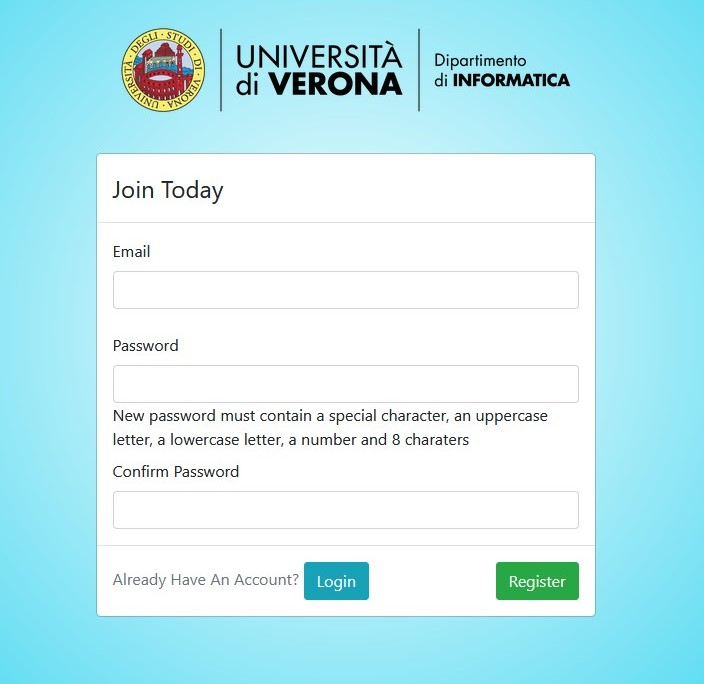
\includegraphics[width=\linewidth]{images/chapter4-flask-register.jpg}
	\caption{Pagina di Registrazione}
\end{minipage}
\hspace{0.5cm}
\end{figure}

\newpage
\subsection{Interfaccia principale}
\label{secsub:flask-funzionalità-principale}
La pagina mostra le opzioni disponibili nel web server.
In alto è presente la barra per eseguire il logout.
All'interno di ogni funzionalità viene mostrata nella barra la possibilità di ritornare nella dashboard.

\begin{figure}[htp]
    \centering
    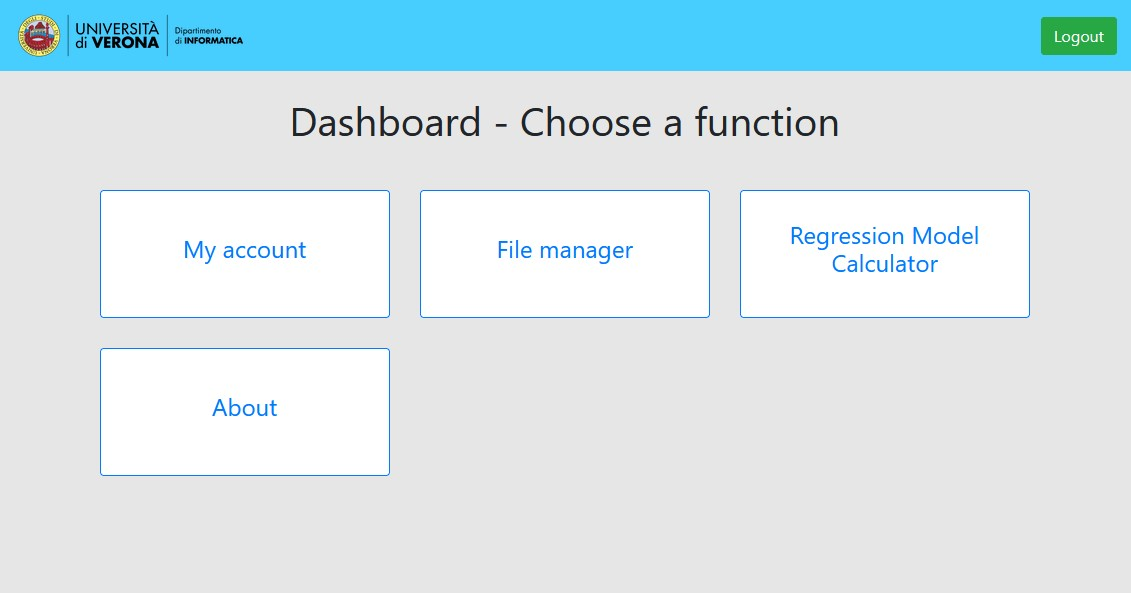
\includegraphics[width=0.85\linewidth]{images/chapter4-flask-daskboard.jpg}
    \caption{Pagina di Dashboard}
\end{figure}

\subsection{Gestione account}
\label{secsub:flask-funzionalità-account}
La pagina permette di cambiare email e password dell'utente connesso.
È possibile modificare solo l'email o la password o entrambi.
Viene mostrala l'email corrente, ma non la password per ragioni di sicurezza.
Quando si inseriscono dei valori si ha la possibilità di premere il tasto per aggiornare i dati.
Se viene superato il controllo del form, viene aggiornato il database e poi viene mostrato il messaggio di avvenuta modifica.
\begin{figure}[htp]
    \centering
    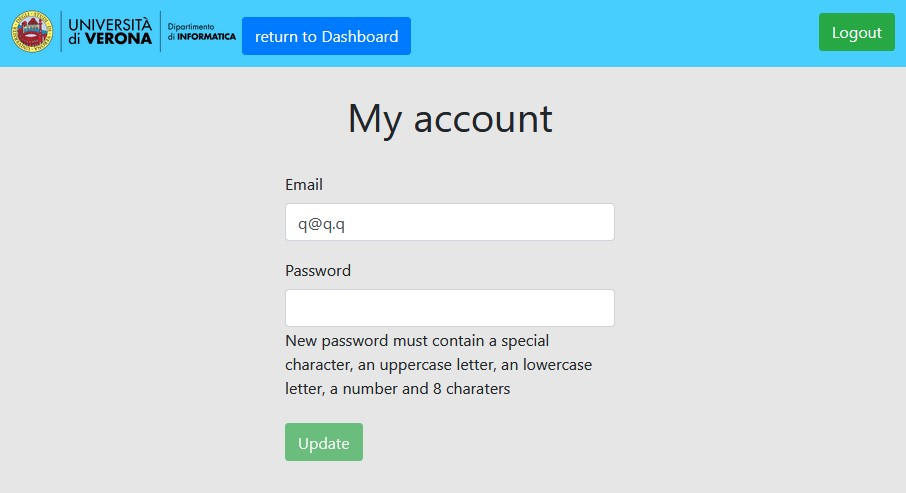
\includegraphics[width=0.85\linewidth]{images/chapter4-flask-myaccount.jpg}
    \caption{Pagina di gestione account}
\end{figure}

\newpage
\subsection{Gestione dei file}
\label{secsub:flask-funzionalità-file}
La pagina permette la gestione delle cartelle e dei file generati con la creazione dei modelli.
L'utilizzo di Javascript ha permesso di implementare la visualizzazione modificando il DOM (Document Object Model),
il quale rappresenta la pagina HTML visualizzata.
Javascript esegue delle chiamate API al server e mostra la lista delle cartelle e dei file richiesti.
Sono state implementate inoltre varie funzionalità, come la possibilità di scaricare un file singolo o l'intera cartella, 
di rinominare e di eliminare file e cartelle.
Nel download è possibile scegliere se scaricare un singolo file oppure una cartella in formato zip.
Le funzioni rinomina e cancella mostrano entrambe una finestra per confermare l'azione che si sta eseguendo.
\begin{figure}[htp]
    \centering
    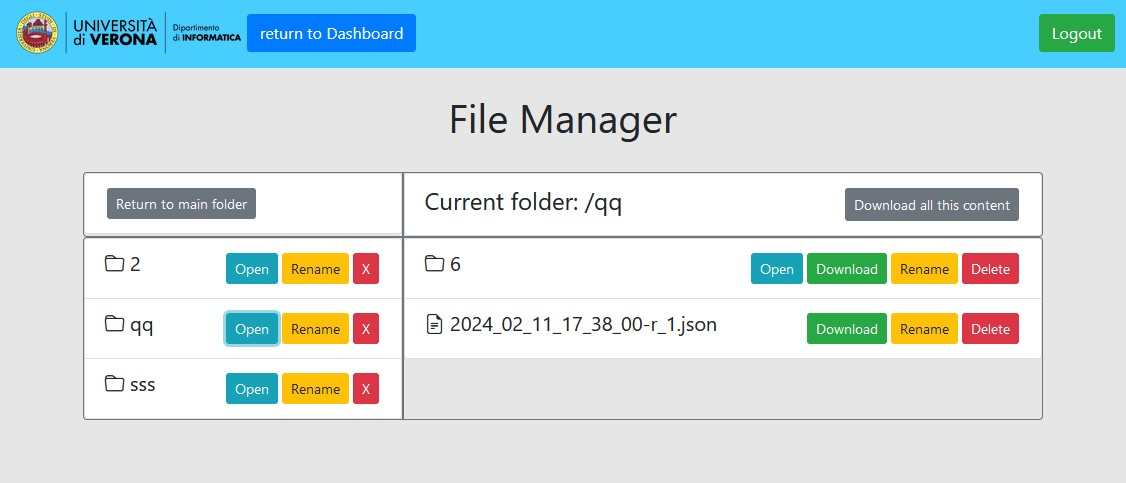
\includegraphics[width=0.85\linewidth]{images/chapter4-flask-file_manager.jpg}
    \caption{Pagina di gestione file}
\end{figure}

\subsection{Creazione dei modelli}
\label{secsub:flask-funzionalità-regressione}
La pagina permette la creazione dei modelli di regressione lineare.
La pagina è stata strutturata in due colonne.
In quella di sinistra è presente il form per l'inserimento dei dati e dei file, 
mentre quella a destra mostra le fasi di elaborazione.
Il form è strutturato nel seguente modo:
\begin{itemize}
	\item \textbf{Model Output Directory}: permette di creare o scegliere una cartella in cui il server salverà
	i file dopo l'esecuzione dello script. La cartella è accessibile tramite la pagina di gestione file.
	\item \textbf{Model Result Name}: permette di specificare quale sarà il nome dei file ottenuti dallo script.
	È un valore opzionale perché in automatico vengono messi sempre come prefisso la data e l'ora corrente.
	\item \textbf{Model Input}: permette di caricare un file in formato CSV contenente i dati storici relativi al sensore. 
	\item \textbf{Model expected output}: permette di caricare uno o più file in formato CSV 
	che rappresentano la variabile di risposta da prevedere.
	\item \textbf{Windows}: è un valore espresso come numero intero non negativo, che
	stabilirà quanti istanti temporali precedenti verranno considerati durante il
	processo di creazione del modello.
	\item \textbf{Test}: permette di scegliere se eseguire il test del modello. 
	In caso affermativo, i dati verranno divisi in addestramento (80\%) e test (20\%) per la verifica della precisione.
\end{itemize}
Una volta terminata la compilazione del form, se i campi necessari sono stati completati viene abilitato il pulsante per inviare i dati.
Se premuto, i dati vengono inviati e viene verificato se soddisfano i requisiti.
Se l'esito è positivo, nella parte destra viene mostrata la fase 1, che dà esito positivo con OK oppure segna ERROR con indicati i campi errati.
Dopo l'esito positivo viene avviata la fase 2 in cui il codice Javascript chiama una API del server per avviare
lo script che esegue la creazione dei modelli. L'utente vedrà un timer e una barra di caricamento nell'attesa.
Al termine dello script il timer si ferma e viene mostrata la fase 3 in cui sono presenti i risultati dell'elaborazione.
Viene anche mostrato un pulsante per andare al gestore dei file.\newline
L'esecuzione dello script può richiedere tempo: per risolvere il problema, l'avvio del calcolo è stato fatto tramite
Javascript in modo che la richiesta non vada in timeout, ma aspetti il termine della computazione.
\begin{figure}[htp]
    \centering
    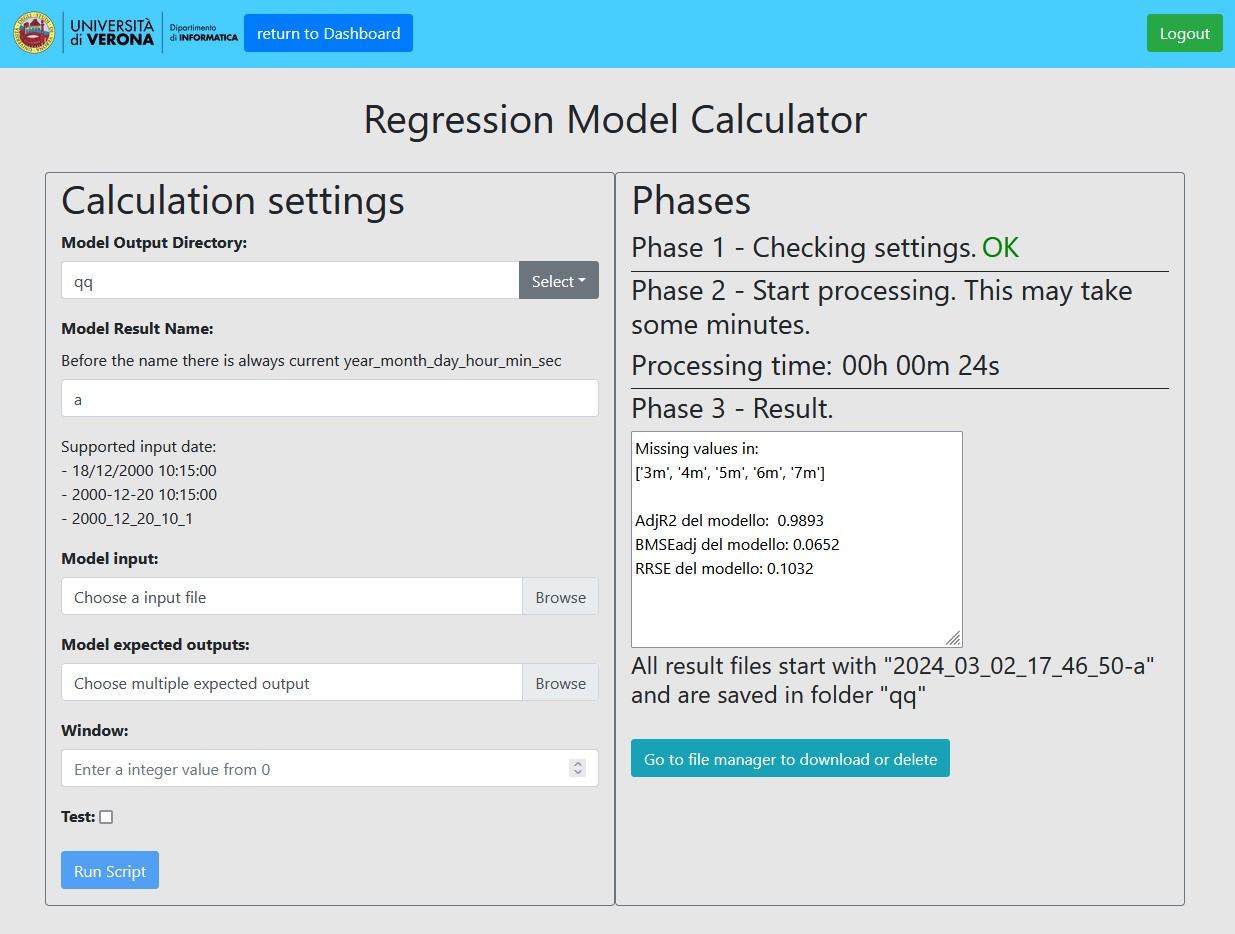
\includegraphics[width=0.7\linewidth]{images/chapter4-flask-regression.jpg}
    \caption{Pagina del calcolo del modello di regressione}
\end{figure}

\newpage
\subsection{Chi siamo}
\label{secsub:flask-funzionalità-about}
In questa pagina sono presenti l'elenco di chi ha collaborato al progetto e le immagini dei volantini presenti alla fiera.
\begin{figure}[htp]
    \centering
    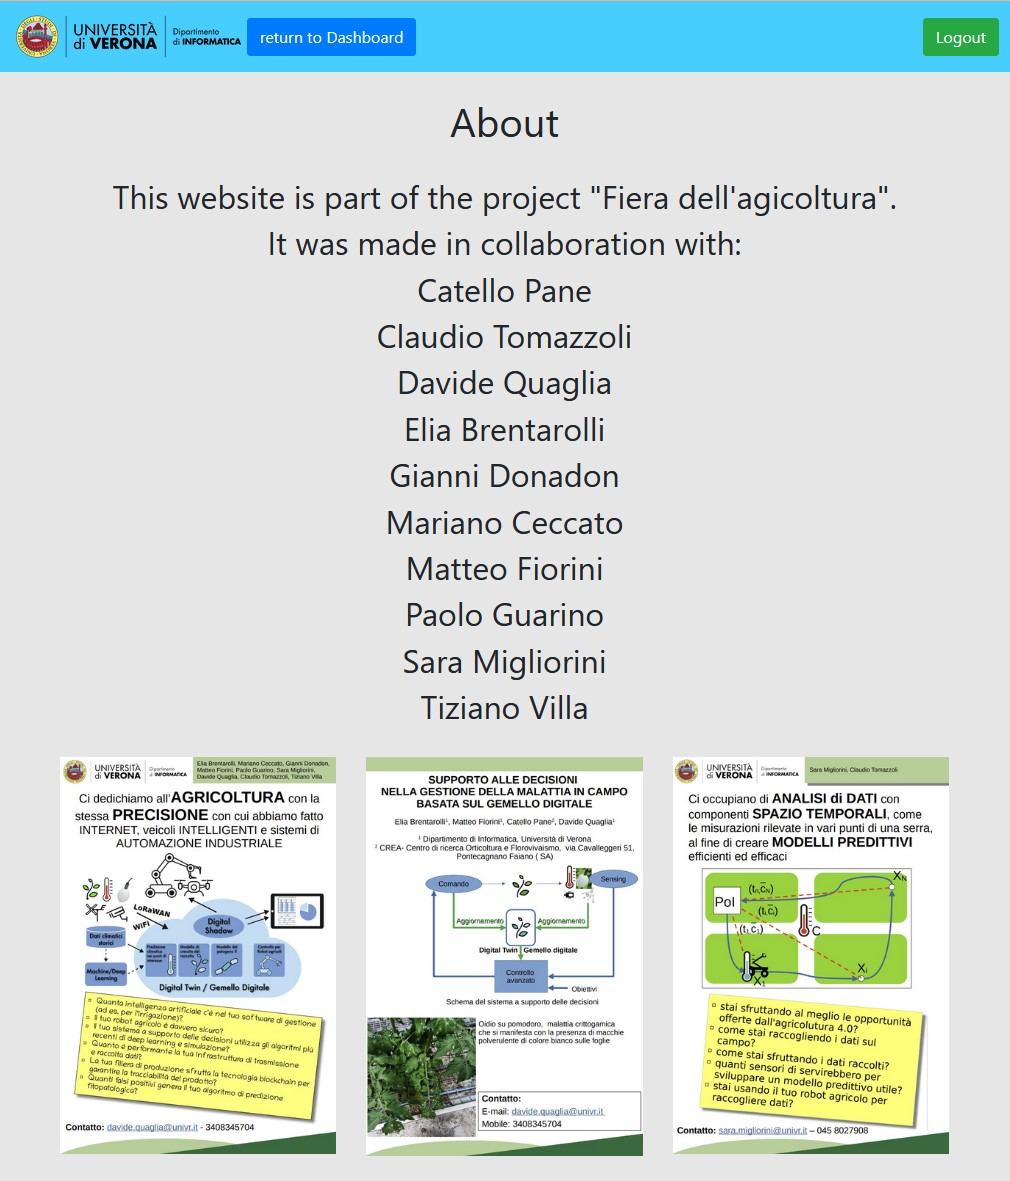
\includegraphics[width=0.7\linewidth]{images/chapter4-flask-about.jpg}
    \caption{Pagina di chi siamo}
\end{figure}

\section{Deployment}
\label{sec:flask-produzione}
Finora il progetto è sempre stato avviato in modalità sviluppo (development).
Tuttavia il server WSGI interno a Flask non è pensato per la messa in esercizio del web server 
quindi si deve usare un altro programma.
Il server WSGI di Flask è sia un server WSGI che un server HTTP, 
quindi si devono trovare due server corrispondenti per il deployment.
Nella documentazione ufficiale vengono elencati alcuni server che si possono usare \cite{flask-doc-deploying}.
Nel progetto è stato usato Gunicorn come server WSGI perché funziona interamente su Python ed è semplice da configurare.
Il server WSGI (Web Server Gateway Interface) è un protocollo di trasmissione che stabilisce e descrive comunicazioni 
ed interazioni tra server ed applicazioni web scritte nel linguaggio Python.
È quindi l'interfaccia standard del web service per la programmazione in Python.
Questo protocollo specifica come i server devono farsi carico delle richieste provenienti dai browser/client e
come devono inoltrare le informazioni richieste alle relative applicazioni, 
oltre a come utilizzare le informazioni di cui si sono fatti carico e come rispondere.
Perciò Gunicorn è il server che si occuperà di eseguire l'applicazione Flask e 
di convertire le richieste HTTP per l'ambiente WSGI e le risposte WSGI in risposte HTTP.
Di questo server si spiegheranno l'installazione e la configurazione.
Manca però il server HTTP che gestisce le richieste e le risposte HTTP.
Nel nostro caso è stato usato NGINX dato che era già presente nella macchina, 
quindi si spiegherà la configurazione necessaria.
Infine si deve impostare Gunicorn per l'avvio automatico tramite Supervisor.

\subsection{Gunicorn}
\label{secsub:flask-produzione-gunicorn}
Di seguito vengono spiegati i comandi usati nel progetto (per i dettagli vedere la documentazione ufficiale \cite{flask-doc-deploying-gunicorn}).
Nello stesso ambiente virtuale in cui si è installato Flask si può installare anche Gunicorn.
Quindi una volta avviato l'ambiente si può procedere con il seguente comando:
\begin{lstlisting}[language=python]
	pip install gunicorn
\end{lstlisting}
Per eseguire il progetto Flask in modalità produzione si deve eseguire il file run\_flask.py tramite Gunicorn.
Il file run\_flask.py è quello commentato nella spiegazione del flusso base \ref{secsub:flask-creazione-basi}
ed è rimasto invariato nelle modifiche del progetto.
Il comando per eseguire tramite Gunicorn è il seguente:
\begin{lstlisting}[language=python]
	gunicorn -w 3 run_flask:app --timeout 0
\end{lstlisting}
I parametri che vengono passati a Gunicorn sono tre.
Il parametro "-w 3" indica quanti processi devono essere avviati per servire il web server.
In questo caso sono indicati 3 processi controllati da Gunicorn che gestiranno le richieste,
così da poter rispondere a più richieste in contemporanea.
Il parametro "run\_flask:app" indica lo script che deve essere eseguito 
e il nome della variabile con cui deve essere eseguito Flask.
Infine il parametro "--timeout 0" indica che i processi di Gunicorn non devono essere interrotti
se l'esecuzione richiede troppo tempo.
L'impostazione a 0, cioè tempo infinito, è stata necessaria dato che l'esecuzione dello script 
di calcolo della regressione può richiedere svariati minuti e il timeout di default è troppo breve.\newline
Per non passare tutti i parametri è possibile creare una configurazione per Gunicorn.
Nel progetto è stata messa nel file gunicorn-config.py ed è la seguente:
\begin{lstlisting}[language=bash]
	bind = '127.0.0.1:8001'
	workers = 3
	timeout = 0
\end{lstlisting}
Oltre ai due parametri precedenti è stato aggiunto quello di bind.
Questo parametro è servito per indicare l'host e su quale porta Gunicorn deve essere in ascolto per le richieste.
Nel progetto si è dovuto specificare che l'host di ascolto è solo locale e che la porta da usare è la numero 8000, 
perché la porta di default 8080 era occupata da un altro servizio.\newline
Per eseguire Gunicorn con il file di configurazione, il comando è:
\begin{lstlisting}[language=python]
	gunicorn -c ./deploy/gunicorn-config.py run_flask:app
\end{lstlisting}
Il server WSGI è stato quindi avviato correttamente.
Per terminarlo basta premere CTRL + C.

\subsection{NGINX}
\label{secsub:flask-produzione-nginx}
Nella macchina su cui si doveva fare l'installazione era già presente NGINX, 
quindi si può fare riferimento alla documentazione ufficiale per l'installazione e i dettagli \cite{flask-doc-deploying-nginx}.
Il file di configurazione per il nostro server web è stato creato nel file nginx-web-server-flask 
(si noti che non ha un'estensione).
La configurazione è la seguente:
\begin{lstlisting}[language=python]
	server {
		listen 8000 ssl;
		server_name mydomain.it;
	
		client_max_body_size 100M;
		
		ssl_certificate /etc/letsencrypt/live/mydomain.it/fullchain.pem;
		ssl_certificate_key /etc/letsencrypt/live/mydomain.it/privkey.pem;
		
		error_page 497 301 =307 https://$server_name:$server_port$request_uri;
	
		location /static {
			alias /path_to_folder/flaskr/static;	
		}
	
		location / {
			proxy_pass http://localhost:8001;
			include /etc/nginx/proxy_params;
			proxy_redirect off;
		}
	
	}
\end{lstlisting}
Nella prima riga viene specificata la porta in ascolto, la 8000, 
e che le richieste devono essere gestite con la sicurezza SSL/TLS.
Poi si indica qual è il nome del dominio del server.
Si specifica la dimensione massima del body contenuto nelle richieste,
che viene impostata a 100 MB dato che è più che sufficiente per le nostre esigenze.
Poi vengono indicati i due path necessari per l'SSL. 
A differenza di Mosquitto qui viene usato il path di riferimento fornito da Certbot, perché
NGINX viene eseguito come utente root quindi non ha problemi ad accedere ai file.
La riga successiva serve per fare il reindirizzamento delle richieste dal protocollo HTTP a HTTPS.
In questo modo si usa sempre una connessione sicura quando si fanno le richieste.
Poi si specificano due locazioni.
La prima serve per fornire i file statici dell'applicazione Flask, 
che vengono richiesti sempre con la prima parte dell'URL formata da /static.
Deve essere specificato il path assoluto della cartella dei file statici.
È anche per questo motivo che sono stati mantenuti tutti i file statici all'interno della cartella static di default,
rendendo accessibile alle richieste dirette solo quella cartella.
La seconda locazione serve invece per girare la richiesta HTTP al server WSGI Gunicorn 
che eseguirà l'applicazione.
La richiesta viene girata tramite il proxy al processo Gunicorn che viene eseguito in locale alla porta 8001.\newline
Una volta creata, la configurazione deve essere spostata nel path delle configurazioni di NGINX, che è il seguente 
(si deve essere root per eseguire questa azione):
\begin{lstlisting}[language=textnonum]
    /etc/nginx/sites-enabled/
\end{lstlisting}
Dopo la copia della configurazione si deve riavviare NGINX con il seguente comando:
\begin{lstlisting}[language=bash]
    sudo systemctl restart nginx
\end{lstlisting}
A questo punto l'applicazione Flask è raggiungibile al dominio indicato alla porta 8000.

\subsection{Avvio automatico di Gunicorn}
\label{secsub:flask-produzione-automatico}
Come ultimo step si deve impostare l'avvio automatico per Gunicorn, 
mentre per NGINX non serve fare nulla perché viene gestito come servizio con systemctl.
Per configurare l'avvio automatico di Gunicorn viene sempre usato Supervisor, visto precedentemente \ref{sec:client-supervisor}.
Viene riportato il file di configurazione:
\begin{lstlisting}[language=bash]
    [program:web-server-flask]
	directory=/home/utente/web-server-flask
	command=/home/utente/web-server-flask/venv/bin/gunicorn -c ./deploy/gunicorn-config.py run_flask:app
	user=utente
	autostart=true
	autorestart=true
	stopasgroup=true
	killasgroup=true
	stderr_logfile=/home/utente/web-server-flask/log/gunicorn/flaskblog.err.log
	stdout_logfile=/home/utente/web-server-flask/log/gunicorn/flaskblog.out.log
\end{lstlisting}
La configurazione segue la spiegazione fornita precedentemente \ref{subsec:client-supervisor-configurazione}.
La cosa più rilevante è il comando che viene passato.
La prima parte indica l'intero path dell'ambiente virtuale in cui è installato Gunicorn. 
Si è dovuto specificare il suo path all'interno dell'ambiente virtuale perché Supervisor non avvia prima l'ambiente virtuale.\newline
Poi si procede con lo spostamento della configurazione \hyperlink{lst:client-supervisor-path}{nella cartella delle configurazioni di Supervisor}.
Infine si eseguono il comando di rilettura configurazione \ref{subsubsec:client-supervisor-rilettura} 
e aggiornamento configurazione \ref{subsubsec:client-supervisor-aggiornamento} per aggiungere
Gunicorn come processo automatico.\newline
Si è quindi terminato tutto il necessario per il deployment. 
Quando la macchina viene riavviata, l'interfaccia web ritorna disponibile. 


%! Author = Gianni
%! Date = 08/02/2024

\chapter{Home Assistant}
\label{ch:homeassistant}

\section{Implementazione nel progetto}
\label{sec:hass-introduzione}
Home Assistant è un software open-source e gratuito per la domotica, 
progettato per essere una piattaforma di integrazione indipendente dall'ecosistema dell'Internet of Things (IoT) 
e un sistema di controllo centrale per i dispositivi smart, 
con particolare attenzione al controllo locale e alla privacy.
Permette di raccogliere i dati provenienti da diversi sensori e di mostrarli in un'interfaccia grafica.
Nel progetto questo software era già installato in una macchina, 
per i dettagli sull'installazione si rimanda alla documentazione ufficiale \cite{hass-installazione}. 
Si doveva solo procedere con la configurazione per ricevere i dati da vari topic del Broker MQTT 
e mostrare i valori in un'interfaccia apposita.
Tuttavia prima viene spiegata una modifica che si è dovuto fare per risolvere un problema con i 
servizi di auto-discovery del software.

\section{Servizi di auto-discovery}
\label{sec:hass-servizi}
Home Assistant fornisce vari servizi tra cui quelli di auto-discovery.
Questi permettono di scoprire nella rete LAN a cui si è connessi le possibili sorgenti dati da integrare nel sistema.
Tuttavia dato che Home Assistant era installato all'interno della rete universitaria,
questi servizi creavano moltissime richieste a causa dell'elevato numero di dispositivi presenti.
È quindi stato necessario modificare la configurazione per disabilitare l'auto-discovery.
La configurazione di Home Assistant si trova all'interno del file configuration.yaml.
Questo file in base al tipo di installazione eseguita può essere modificato da interfaccia grafica o
da riga di comando.
Nel nostro caso l'installazione è stata fatta tramite container Docker, 
quindi il file di configurazione era modificabile da riga di comando e si trovava nella seguente cartella:
\begin{lstlisting}[language=textnonum]
    /var/docker
\end{lstlisting}
Nel file è presente di default la seguente configurazione:
\begin{lstlisting}[language=textnonum]
    default_config:
\end{lstlisting}
Con questa configurazione si abilitano usa serie di componenti che di solito sono utili per semplificare l'uso
del software, tra cui quelli di auto-discovery.
Per risolvere il problema è stata commentata quella configurazione 
e sono state aggiunte tutte le configurazioni a cui corrispondeva disabilitando quelle di auto-discovery.
In base alla versione di Home Assistant, 
la configurazione può corrispondere a un numero maggiore o minore di servizi.
In questa installazione era presente la versione 2023.3.1 
e quel parametro corrispondeva ai seguenti servizi:
\begin{lstlisting}[language=bash]
    #automation: !include automations.yaml ALREADY PRESENT 
    backup:
    bluetooth:
    #cloud:
    config:
    counter:
    #dhcp:
    energy:
    #frontend: ALREADY PRESENT 
    hardware:
    history:
    homeassistant_alerts:
    image:
    input_boolean:
    input_button:
    input_datetime:
    input_number:
    input_select:
    input_text:
    logbook:
    map:
    media_source:
    mobile_app:
    my:
    #network:
    person:
    schedule:
    #scene: !include scenes.yaml ALREADY PRESENT 
    #script: !include scripts.yaml ALREADY PRESENT 
    #ssdp:
    #stream:
    sun:
    system_health:
    tag:
    timer:
    usb:
    webhook:
    #zeroconf:
    zone:
\end{lstlisting}
I parametri che hanno un cancelletto davanti sono disattivati.
I parametri seguiti da ALREADY PRESENT 
sono stati attivati in modo diverso da un'altra parte nel file della configurazione.
I parametri importanti da disattivare erano cloud, dhcp, network, ssdp, stream e zeroconf.
In questo modo sono stati disabilitato completamente i servizi di auto-discovery 
e sono state ridotte al minimo le richieste che Home Assistant eseguiva nella rete.
Si rimanda alla documentazione per sapere il significato di ogni parametro \cite{hass-config}.
Nella community di Home Assistant ci sono state altre persone 
che hanno dovuto affrontare lo stesso problema, 
riporto alcuni casi che mi sono stati utili \cite{hass-config-community1} \cite{hass-config-comumnity2}.

\section{Integrazione con MQTT}
\label{sec:hass-MQTT}
Per far ricevere a Home Assistant i messaggi del broker MQTT si devono fare due passaggi.
Il primo è configurare il client per connettersi al broker 
e il secondo è definire un sensore per ogni valore presente nel messaggio in arrivo dal Broker.
Per configurare il client si deve eseguire la procedura da interfaccia web, 
come spiegato nella documentazione \cite{hass-mqtt}.
Quindi per inserire la configurazione si deve andare in "Impostazioni", poi "dispositivi e servizi",
premere in basso a destra il pulsante + e selezionare dalla lista "MQTT".
A questo punto si apre una finestra che deve essere popolata con la configurazione per la connessione
come se fosse un normale client MQTT.
La configurazione usata nel progetto è la seguente:
\begin{lstlisting}[language=textnonum]
    broker: mydomain.it
    port: 8883
    username: username
    password: password
    client ID: (vuoto)
    time: (60 il valore di default)
    Usa un certificato client: False
    Convalida del certificato: automatico
    Ignora la convalida del certificato del broker: True
    Protocollo MQTT: 3.1.1
    Trasporto MQTT: TCP
\end{lstlisting}
Poi si preme su avanti e si segue le richieste fino a completare la procedura.
Si è quindi configurato il client che riceve i messaggi.
Home Assistant supporta la configurazione di un broker alla volta.
Nel secondo passaggio si deve modificare il file configuration.yaml per aggiungere i vari sensori.
Nel file si deve aggiungere ad esempio il seguente codice:
\begin{lstlisting}[language=bash]
    mqtt:
        sensor:
            - name: Serra reale Temperatura Aria
              state_topic: sensori
              unique_id: sensor.reali.serraAirTemperature
              unit_of_measurement: "°C"
              value_template: >
              
                  {{ value_json.Temp__C }}
              
                  {{ sensor.reali.serraAirTemperature }}
              
\end{lstlisting}
La prima riga indica che il sensore che si sta aggiungendo ha come sorgente il broker MQTT.
Poi nella seconda lista si specifica di che tipo è il sensore, 
in questo caso è indicato un semplice sensore.
Poi si definisce il sensore iniziando la dichiarazione con "- ".
Viene indicato il nome visualizzato nell'interfaccia grafica, il topic da cui prendere il messaggio,
un id unico per identificare il sensore, 
l'unità di misura e infine come il valore deve essere visualizzato.
Nel campo valore è possibile definire la logica per eseguire controlli, modifiche o altro 
per ottenere il valore finale.
Per aggiungere altri sensori, basta inserire altre definizioni prestando attenzione all'indentazione
e ricordandosi di mettere "- " prima della definizione.
Nell'appendice vengono riportati altri esempi di definizioni di sensori~\ref{sec:hass-appendix-sensori}.

\section{Visualizzazione dei dati}
\label{sec:hass-visualizzazione}
Per configurare come vengono visualizzati i dati, si deve agire da interfaccia grafica.
Come prima cosa si deve creare una nuova plancia (in inglese dashboard).
Si deve andare in "Impostazioni", poi "Plance" e in basso a sinistra premere su +.
Si apre una finestra in cui si deve mettere il nome della plancia, un'icona, l'URL e altre impostazioni.
Una volta configurato, si preme su crea e nella barra a sinistra si aggiungerà la nuova plancia.
Successivamente si può iniziare a configurare la visualizzazione,
si consiglia di guardare la documentazione per tutte le possibilità di personalizzazione \cite{hass-dashboard}.
Si va nella plancia appena creata, in alto a destra si apre il menù e si seleziona "modifica plancia".
Poi si clicca di nuovo sul menù in alto a destra e si seleziona "Editor di configurazione testuale".
Viene visualizzato un file simile a quello di configurazione.
Di seguito viene riportata una parte della configurazione di una plancia:
\begin{lstlisting}[language=bash]
    title: Oidio
    background: center / cover no-repeat fixed url('/local/background_verde_sfumature.jpg')
    views:
      - theme: Backend-selected
        title: Normale
        icon: ''
        path: normale
        badges: []
        cards:
          - type: vertical-stack
            cards:
              - type: entities
                title: Riepilogo Sensori
                entities:
                  - entity: sensor.serra_reale_temperatura_aria
                    name: Temperatura Aria
          - type: vertical-stack
            cards:
              - type: picture-elements
                title: Stime Rischio Oidio
                image: http://mydomain.it:8123/local/Mappa_new.png
                elements:
                  - type: state-badge
                    entity: sensor.serra_stima_oidio_rischio_1
                    style:
                      top: 28%
                      left: 37%
                      scale: 90%
                      color: rgba(0,0,0,0)
\end{lstlisting}
Nella configurazione alla prima riga c'è il nome della plancia.
La seconda riga definisce il background che deve avere la plancia.
L'immagine è salvata in una cartella accessibile da Home Assistant che è 
\begin{lstlisting}[language=textnonum]
    /var/docker/www
\end{lstlisting}
Poi viene definita una scheda della plancia con il tema, il titolo, nessuna icona e il path dell'URL.
Poi si definiscono le cards, che sono i gruppi di elementi che devono essere mostrati.
Il primo gruppo viene definito come un insieme di card verticali.
Al suo interno c'è una card che contiene entità e ha nome "Riepilogo sensori".
Le entità in questo caso sono solo una: un sensore identificato da un nome univoco e il nome visualizzato.
Anche il secondo gruppo è un insieme di card verticali.
Contiene una card di tipo immagine-elementi che permette di visualizzare un'immagine 
con sopra i valori dei sensori.
Viene impostato il titolo, l'immagine in background e la lista di elementi.
L'immagine è sempre contenuta nella cartella del background.
Gli elementi in questo caso sono solo uno, che è di tipo badge.
Viene specificato il nome univoco del sensore da cui prendere i dati
e vengono definiti degli stili del badge.
Nell'appendice vengono riportate le definizioni usate~\ref{sec:hass-appendix-plancia}.
Una volta terminata l'impostazione delle varie card e delle relative sorgenti, 
si preme "salva" in alto a destra e poi su "fatto".
In questo modo si è ottenuta la visualizzazione di due sensori con sorgente MQTT modificando la plancia.\newline
Di seguito viene riportata l'immagine di uno dei risultati che è stato raggiunto 
modificando opportunamente questo file.

\begin{figure}[htp]
    \centering
    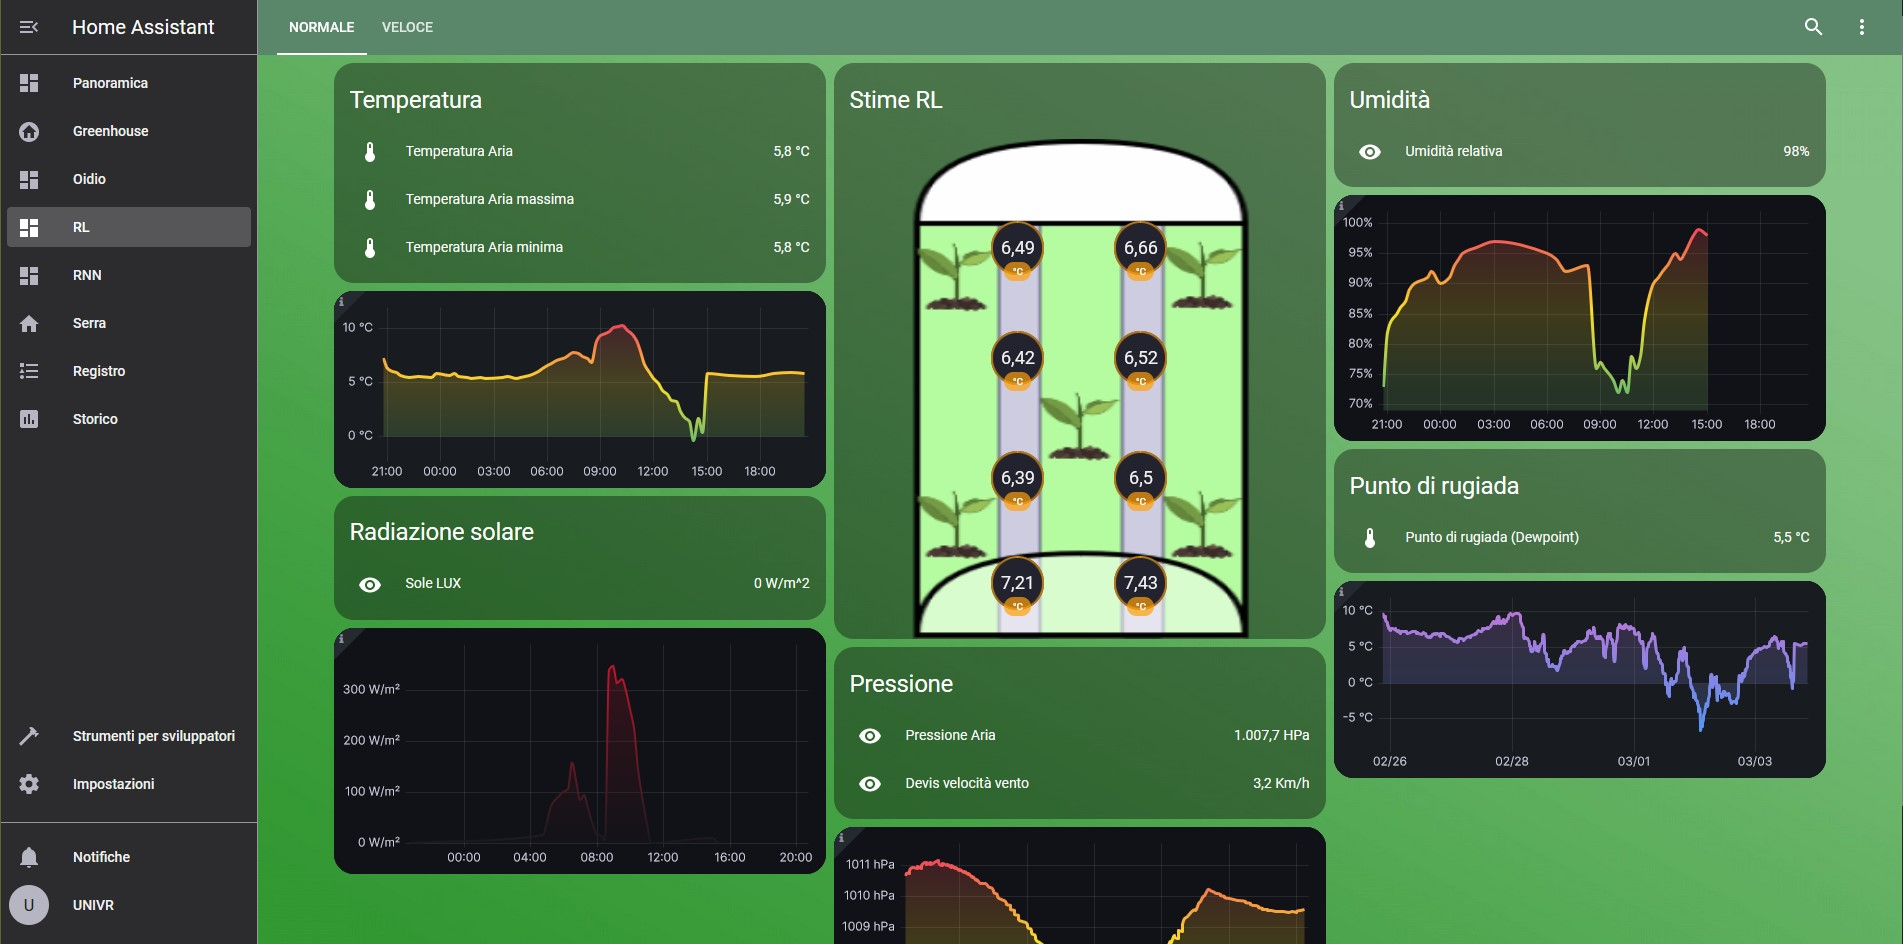
\includegraphics[width=1\linewidth]{images/chapter5-hass-visualizzazione.jpg}
    \caption{Plancia RL}
\end{figure}

%! Author = Gianni
%! Date = 08/02/2024

\chapter*{Conclusioni}
\addcontentsline{toc}{chapter}{\protect\numberline{}Conclusioni}

Lo svolgimento del progetto mi ha permesso di applicare varie conoscenze 
apprese durante gli anni universitari.
Da un lato ho potuto sperimentare la programmazione di complessi script Python
e dall'altro ho potuto agire come sistemista per far collaborare tutti i vari componenti.\newline
\newline
Alla base del progetto c'è il broker MQTT che fa da ponte per i dati tra le varie parti.
Tutto parte dall'emulazione di sensori reali che viene fatta da alcuni client MQTT che pubblicano dati.
Tramite l'interfaccia web vengono generati i modelli di elaborazione dei dati dei sensori.
Questi modelli vengono usati da altri client MQTT per generare nuovi dati
a partire dai sensori emulati.
Infine con Home Assistant è possibile vedere in un'interfaccia grafica tutti i dati 
che vengono pubblicati sul broker.\newline
\newline
È possibile scaricare il codice sviluppato dalla repository GitHub
al \href{https://github.com/aletkw00/models_calculator/tree/masterG-python36}{seguente link}.



\chapter*{Ringraziamenti}
\addcontentsline{toc}{chapter}{\protect\numberline{}Ringraziamenti}
Giunto alla conclusione di questa tesi voglio ringraziare una persona molto speciale,
la dottoressa Cristina Calonego, l'amore della mia vita.
Lei mi ha supportato in tutte le varie fasi del mio percorso universitario
motivandomi a studiare e a portare a termine il percorso.
Inoltre mi ha aiutato a revisionare questa tesi per renderla comprensibile a tutti
e per controllare che non ci fossero porcherie grammaticali.
Ringrazio la mia famiglia che mi ha supportato economicamente e moralmente
in questi anni nonostante tutte le mie insicurezze.
Infine voglio ringraziare il Prof. Davide Quaglia e il Dott. Elia Brentarolli per 
avermi dato la possibilità di partecipare a questo progetto 
che è stato presentato alla Fieragricola 2024 di Verona.



\appendix

%! Author = Gianni
%! Date = 17/10/2023


\chapter{Configurazioni broker MQTT}
\label{ch:broker-configurazioni-broker-mqtt}

\section{/mosquitto.conf}
\label{sec:/mosquitto.conf}
Questa configurazione è quella che mosquitto dovrebbe creare al momento dell'installazione.
Se non è presente potrebbe non funzionare.\newline
Il seguente file deve essere inserito in \textbf{/etc/mosquitto}.
\begin{lstlisting}[caption={mosquitto.conf},language=text]
# Place your local configuration in /etc/mosquitto/conf.d/
#
# A full description of the configuration file is at
# /usr/share/doc/mosquitto/examples/mosquitto.conf.example

pid_file /var/run/mosquitto.pid

persistence true
persistence_location /var/lib/mosquitto/

log_dest file /var/log/mosquitto/mosquitto.log

include_dir /etc/mosquitto/conf.d
\end{lstlisting}

\section{/conf.d/localhost-TLS.config}
\label{sec:/conf.d/localhost-tls.config}
Questa configurazione è quella creata ad hoc.
Ha 2 listener separati, uno per localhost con accesso libero, uno per tutti con accesso tramite
credenziali e connessione tramite SSL/TLS.\newline
Il seguente file deve essere inserito in \textbf{/etc/mosquitto/conf.d}.
\begin{lstlisting}[caption={mosquitto.conf},language=text]
# abilita differenti configurazioni per listener
per_listener_settings true
#
# per accesso solo locale e libero
listener 1883 localhost
allow_anonymous true
#
# per accesso con credenziali e certificato SSL/TLS
listener 8883
allow_anonymous false
password_file /etc/mosquitto/passwordfile
certfile /etc/mosquitto/certs/fullchain.pem
keyfile /etc/mosquitto/certs/privkey.pem
\end{lstlisting}

\section{Script rinnovo certificati}
\label{sec:script-rinnovo-certificati}
Questo script deve essere messo nella cartella /etc/letsencrypt/renewal-hooks/deploy/ e reso eseguibile.
Copia i certificati del dominio inserito nella cartella /etc/mosquitto/certs/ in modo che Mosquitto possa accedervi.
Quando copia, invia a Mosquitto un segnale per ricaricare i certificati.
\begin{lstlisting}[caption={mosquitto-copy.sh},language=text]
#!/bin/sh

# This is an example deploy renewal hook for certbot that copies newly updated
# certificates to the Mosquitto certificates directory and sets the ownership
# and permissions so only the mosquitto user can access them, then signals
# Mosquitto to reload certificates.

# RENEWED_DOMAINS will match the domains being renewed for that certificate, so
# may be just "example.com", or multiple domains "www.example.com example.com"
# depending on your certificate.

# Place this script in /etc/letsencrypt/renewal-hooks/deploy/ and make it
# executable after editing it to your needs.

# Set which domain this script will be run for
MY_DOMAIN=example.com
# Set the directory that the certificates will be copied to.
CERTIFICATE_DIR=/etc/mosquitto/certs

for D in ${RENEWED_DOMAINS}; do
	if [ "${D}" = "${MY_DOMAIN}" ]; then
		# Copy new certificate to Mosquitto directory
		cp ${RENEWED_LINEAGE}/fullchain.pem ${CERTIFICATE_DIR}/server.pem
		cp ${RENEWED_LINEAGE}/privkey.pem ${CERTIFICATE_DIR}/server.key

		# Set ownership to Mosquitto
		chown mosquitto: ${CERTIFICATE_DIR}/server.pem ${CERTIFICATE_DIR}/server.key

		# Ensure permissions are restrictive
		chmod 0600 ${CERTIFICATE_DIR}/server.pem ${CERTIFICATE_DIR}/server.key

		# Tell Mosquitto to reload certificates and configuration
		pkill -HUP -x mosquitto
	fi
done
\end{lstlisting}

%! Author = Gianni
%! Date = 17/10/2023


\chapter{Skeleton client MQTT}
\label{ch:client-appendix}

\section*{config.py}
\label{sec:client-appendix-subpub-conf}
File di configurazione per lo script principale.
\begin{lstlisting}[language=bash]
    """
    Configurazione 
    """
    
    # Config. per connessione
    HOST = 'host'
    USER = 'user'
    PASSWORD = 'pass'
    CERT_TLS = 'ISRG_Root_X1.pem'
    
    # Nomi dei topic ricezione
    TOPIC_RECEIVE_1 = "topic1"
    TOPIC_RECEIVE_2 = "topic2"
    
    # Nome topic invio
    TOPIC_SEND_1 = "topic3"
    TOPIC_SEND_2 = "topic4"
\end{lstlisting}

\section*{subscriber\_e\_publisher.py}
\label{sec:client-appendix-subpub-main}
File principale in cui ci si iscrive a dei topic.
Alla ricezione di messaggi si elaborano e poi si pubblica il risultato.
\begin{lstlisting}[language=bash]
    import paho.mqtt.client as mqtt
    import json
    
    import config
      
    #------------------------
    # CLASSE PER I PARAMETRI
    #
    class configurazione_localhost:
        def __init__(self, topic_ricezione_1, topic_ricezione_2, topic_invio_1, topic_invio_2):
            self.dizionario = {"host": "localhost",
                               "porta": 1883,
                               "login": False,
                               "username": "",
                               "password": "",
                               "topic-ricezione-1": topic_ricezione_1,
                               "topic-ricezione-2": topic_ricezione_2,
                               "topic-invio-1": topic_invio_1,
                               "topic-invio-2": topic_invio_2,
                               "cert_tls": ''}
        
        def aggiorna_ad_esterna_login_tls(self, host, username, password, nome_cert):
            self.dizionario.update({"host": host})
            self.dizionario.update({"porta": 8883})
            self.dizionario.update({"login": True})
            self.dizionario.update({"username": username})
            self.dizionario.update({"password": password})
            self.dizionario.update({"cert_tls": nome_cert})
    
        def get_host(self): 
            return self.dizionario.get('host')
        
        def get_porta(self):
            return int(self.dizionario.get('porta'))
    
        def get_login(self):
            return bool(self.dizionario.get('login'))
    
        def get_username(self):
            return self.dizionario.get('username')
    
        def get_password(self):
            return self.dizionario.get('password')
    
        def get_topic_ric_1(self):
            return self.dizionario.get('topic-ricezione-1')
            
        def get_topic_ric_2(self):
            return self.dizionario.get('topic-ricezione-2')
        
        def get_topic_inv_1(self):
            return self.dizionario.get('topic-invio-1')
        
        def get_topic_inv_2(self):
            return self.dizionario.get('topic-invio-2')
        
        def get_cert_tls(self):
            return self.dizionario.get('cert_tls')
    
    #-------------------------------------
    # FUNZIONE PER LA ELABORAZIONE ALLA RECEZIONE DI UN MESSAGGIO
    # L'output deve essere un json/dizionario
    #
    def elaborazione(msg, topic, par):
        global variabile_globale_1
        global variabile_globale_2
        
        # DEBUG - Stampa tutto il contenuto del messaggio
        # print(msg)
        
        # Converte il messaggio in un json (dizionario)
        msg_json = json.loads(msg)
    
    
        # Esegue il dump del json
        nuovo_msg = json.dumps(msg_json)
        
        # TOGLIERE IL COMMENTO PER DEBUG
        # print(nuovo_msg) 
        return nuovo_msg
    
    #----------------------------------
    # CLIENT MQTT
    # definizione di cosa deve fare alla connessione, iscrizione, ricezione, invio, log
    #
    def sub_pub_mqtt(par: configurazione_localhost):
    
        def on_connect(client, userdata, flags, rc):
            # TOGLIERE IL COMMENTO PER DEBUG
            # print(client, userdata, flags, rc)
            pass
    
        def on_subscribe(client, userdata, mid, granted_qos):
            # TOGLIERE IL COMMENTO PER DEBUG
            # print("message topic=", mid)
            # print("message qos=", granted_qos)
            pass
    
        def on_message(client, userdata, msg):
            json_string = elaborazione(msg.payload.decode(), msg.topic, par)
    
            if json_string:  
                client_pub_sub.publish(
                    topic=par.get_topic_inv_1(),
                    payload=json_string,
                    retain=True
                )        
    
        def on_log(client, userdata, level, buf):
            print("log: ", buf)
    
        # crea il client per la connessione
        client_pub_sub = mqtt.Client(
            client_id=None,
            clean_session=True,
            userdata=None,
            protocol=mqtt.MQTTv311,
            transport='tcp'
        )
    
        # callback
        client_pub_sub.on_connect = on_connect  # si puo' commentare se non interessa
        client_pub_sub.on_subscribe = on_subscribe  # si puo' commentare se non interessa
        client_pub_sub.on_message = on_message
        # --------------------- 
        # PER DEBUG
        # da commentare per non vedere i log
        #client_pub_sub.on_log = on_log
    
        # controlla se c'e' il login
        if par.get_login():
            client_pub_sub.username_pw_set(par.get_username(), par.get_password())
    
        # controlla la porta di invio e setta il certificato
        if par.get_porta() != 1883:
            client_pub_sub.tls_set(ca_certs=par.get_cert_tls(), tls_version=2)
    
        # esegue la connessione al broker
        client_pub_sub.connect(
            host=par.get_host(),
            port=par.get_porta(),
            keepalive=60
        )
    
        # Iscrizione ai topic di ricezione
        client_pub_sub.subscribe(topic=par.get_topic_ric_1())
        # CI SI PUO' ISCRIVERE A PIU' TOPIC
        # client_pub_sub.subscribe(topic=par.get_topic_ric_2())
    
        # attesa dei messaggi all'infinito, serve per eseguire i callback
        client_pub_sub.loop_forever(timeout=1.0, max_packets=1, retry_first_connection=False)

    #-------------------------------------------
    # FUNZIONE MAIN
    if __name__ == "__main__":
    
        # definizione di variabili globali
        global variabile_globale_1
        global variabile_globale_2
        
        variabile_globale_1  = False
        variabile_globale_2 = False
        
        # Connessione al broker e avvio del client mqtt
        parametri = configurazione_localhost(config.TOPIC_RECEIVE_1, config.TOPIC_RECEIVE_2, config.TOPIC_SEND_1, config.TOPIC_SEND_2)
        #
        # togliere il commento per configurazione esterna alla macchina
        #parametri.aggiorna_ad_esterna_login_tls(config.HOST, config.USER, config.PASSWORD, config.CERT_TLS)
    
        sub_pub_mqtt(parametri)
\end{lstlisting}

%! Author = Gianni
%! Date = 17/10/2023


\chapter{Configurazioni Home Assistant}
\label{ch:hass-appendix}


\section{Definizioni di sensori MQTT}
\label{sec:hass-appendix-sensori}
Qui sono riportate le definizioni di sensori MQTT 
usate nel file configuration.yaml.

\subsection*{Sensore con valore semplice}
\label{sec:hass-appendix-sensori-normali}
La configurazione di un sensore con valore numerico intero. 
\begin{lstlisting}[language=bash]
    - name: Serra reale Temperatura Aria
      state_topic: sensori
      unique_id: sensor.reali.serraAirTemperature
      unit_of_measurement: "°C"
      value_template: >
        
          {{ value_json.Temp__C }}
        
          {{ sensor.reali.serraAirTemperature }}
        
\end{lstlisting}


\subsection*{Sensore con valore arrotondato}
\label{sec:hass-appendix-sensori-float}
La configurazione di un sensore con valore numerico con la virgola 
che viene arrotondato alla seconda cifra decimale.
\begin{lstlisting}[language=bash]
    - name: Serra stima RL Temperatura 1
      state_topic: sensori/modelliRL
      unique_id: sensor.PredRL.serraTemperatura_1
      unit_of_measurement: "°C"
      value_template: >
        
          {{ value_json.RL_1 | float | round(2) }}
        
          {{ sensor.PredRL.serraTemperatura_1 }}
        
\end{lstlisting}


\section{Definizioni di cards}
\label{sec:hass-appendix-plancia}
Di seguito viene riportato il codice usato per la creazione
delle card nell'interfaccia grafica.

\subsection*{Card per le entità}
\label{sec:hass-appendix-plancia-entità}
Permette di mostrare il nome e il valore del sensore.
\begin{lstlisting}[language=bash]
    - type: entities
      title: Temperatura
      entities:
        - entity: sensor.serra_reale_temperatura_aria
          name: Temperatura Aria
        - entity: sensor.serra_reale_massima_temperatura_aria
          name: Temperatura Aria massima
        - entity: sensor.serra_reale_minima_temperatura_aria
          name: Temperatura Aria minima    
\end{lstlisting}

\subsection*{Card per immagini-elementi}
\label{sec:hass-appendix-plancia-pic-ele}
Permette di mostrare un'immagine con sopra dei badge 
che contengono i valori dei sensori.
\begin{lstlisting}[language=bash]
    - type: picture-elements
      title: Stime RL
      image: http://mydomain.it:8123/local/Mappa_new.png
      elements:
        - type: state-badge
          entity: sensor.serra_stima_rl_temperatura_1
          style:
            top: 28%
            left: 37%
            scale: 95%
            color: rgba(0,0,0,0)
        - type: state-badge
          entity: sensor.serra_stima_rl_temperatura_3
          style:
            top: 50%
            left: 37%
            scale: 95%
            color: rgba(0,0,0,0)
        - type: state-badge
          entity: sensor.serra_stima_rl_temperatura_5
          style:
            top: 74%
            left: 37%
            scale: 95%
            color: rgba(0,0,0,0)
        - type: state-badge
          entity: sensor.serra_stima_rl_temperatura_7
          style:
            top: 95%
            left: 37%
            scale: 95%
            color: rgba(0,0,0,0)
        - type: state-badge
          entity: sensor.serra_stima_rl_temperatura_2
          style:
            top: 28%
            left: 62%
            scale: 95%
            color: rgba(0,0,0,0)
        - type: state-badge
          entity: sensor.serra_stima_rl_temperatura_4
          style:
            top: 50%
            left: 62%
            scale: 95%
            color: rgba(0,0,0,0)
        - type: state-badge
          entity: sensor.serra_stima_rl_temperatura_6
          style:
            top: 74%
            left: 62%
            scale: 95%
            color: rgba(0,0,0,0)
        - type: state-badge
          entity: sensor.serra_stima_rl_temperatura_8
          style:
            top: 95%
            left: 62%
            scale: 95%
            color: rgba(0,0,0,0)
\end{lstlisting}

\subsection*{Card per iframe}
\label{sec:hass-appendix-plancia-iframe}
Permette di mostrare una pagina web all'interno di un elemento.
È stato usato per inserire i grafici di Grafana.
\begin{lstlisting}[language=bash]
    - type: iframe
      url: >- url_to_web_page_to_embed
      aspect_ratio: 40% 
\end{lstlisting}

\bibliographystyle{plain}
\bibliography{bibliography}

\end{document}
